%!TEX root = ..\..\main.tex
\chapter{Maximum Likelihood Location Mixtures}
\label{Ch:Mixtures}

\lhead{Chapter \ref{Ch:Mixtures}. \emph{Maximum Likelihood Location Mixtures}}

\graphicspath{{Figures/Mixtures/}}

%-------------------------------------------------------------------------------
%	Chapter Text
%-------------------------------------------------------------------------------

\section{Introduction}
	Mixtures of distributions have been used to model a wide variety of phenomena, with successful applications in the fields of ``astronomy, biology, genetics, medicine, psychiatry, economics, engineering, and marketing, among many other fields in the biological, physical, and social sciences'' \cite[Section 1.1.1]{McLachlan2004-ik}. Mixture models have been in use for over 100 years. In 1894, Pearson used a mixture of two normal densities to model the distribution of the ratio of forehead to body lengths of a sample of 1000 crabs \cite{Pearson1894-qv}. His mixture of two normals was able to account for the skewness in the data, which a single normal could not model. Pearson suggested that this signalled the existence of two sub-populations of crabs; each associated with its own normal distribution.

	However, we do not require that data comes from a mixture of distributions in any physical sense for mixtures to be a useful modelling tool. 
	One of the traits that has contributed to the extent of the use of mixtures is that they provide a convenient semi-parametric way of modelling unknown distributions. They are particularly useful in situations where a parametric method is too restrictive to satisfactorily model the data, and a fully non-parametric method, such as kernel density estimation, may require evaluating a sum which contains more terms than desired. By way of illustration, Priebe in \cite{Priebe1994-ng} discussed modelling a log normal density using a mixture of normals. With $n = 10000$ observations, Priebe only required about 30 normals to obtain a good approximation. This is in contrast to a kernel density estimator which would contain 10000 terms.

	% [WHAT ELSE?]

	% \subsection{Definitions}
	A \emph{mixture density} is a probability density function that can be written in the form
	\begin{equation}
		f_Q(\vect{x}) = \int_\Omega f(\vect{x}; \vect{\theta}) \intd Q(\vect{\theta}),
		\label{eq:mixture definition}
	\end{equation}
	where $f(\vect{x};\vect{\theta})$ is the \emph{component density}, parametrised by $\vect{\theta} \in \Omega$, and $Q$ is a probability distribution on $\Omega$, called the \emph{mixing distribution}. In the case that $Q$ is a discrete probability distribution, with probability masses $p_j$ at points $\vect{\theta}_j$, $j = 1, \dots, m$, the mixture density in \eqref{eq:mixture definition} is a \emph{finite mixture} and can be written
	\begin{equation}
		f_Q(\vect{x}) = f_{\vect{\theta}, \vect{p}}(\vect{x}) = \sum_{j = 1}^m p_j f(\vect{x}; \vect{\theta}_j).
	\end{equation}

	In this chapter, we will be concerned only with finite mixtures on the real line, whose component densities are parametrised by a single shifting parameter, $\theta$ (we may of course allow for other fixed parameters, for example normal distributions with varying locations but fixed variance). This is what we will call a \emph{location mixture}, and it can be written as
	\begin{equation}
		f_{\vect{p}, \vect{\theta}} = \sum_{j = 1}^m p_j f(x - \theta_j)
		\label{eq:location mixture}
	\end{equation}
	for a single component density $f(x)$.
	Looking only at mixtures of this form is not as restrictive as it may at first seem. Using a finite location mixture of normals, one can approximate any continuous density arbitrarily well \cite{Nguyen2018-qx}.

	A common question when using mixtures is the following. Let $\vect{X} = (X_1, \dots, X_n)$ be a set of independent and identically distributed random variables, where each $X_i$ has probability density function $g(\vect{x})$. Given $\vect{x} = (x_1, \dots, x_n)$, an observed random sample of $\vect{X}$, and a component density $f(\vect{x}; \vect{\theta})$, how do we choose the mixing distribution $Q$ so that $f_Q(\vect{x})$ is a good approximation for $g(\vect{x})$?	One answer to this question is to choose $Q$ to maximise the likelihood.

	The \emph{likelihood} of a distribution $Q$ given $\vect{x}$ is 
	\begin{equation}
		L(Q;\vect{x}, f) = \prod_{i = 1}^n f_Q(x_i).
	\end{equation}
	Maximizing $L(Q;\vect{x}, f)$ may be achieved by instead maximizing the \emph{log likelihood},
	\begin{equation}
		l(Q; \vect{x}, f) = \log L(Q; \vect{x}, f) = \sum_{i = 1}^n \log f_Q(x_i),
		\label{eq:loglikelihood}
	\end{equation}
	since $\log(x)$ is a strictly increasing function. In \cite{Lindsay1983-tf}, Lindsay showed that provided that the likelihood is bounded, there exists a maximizing $Q$ that has at most $n$ points of support. This is a useful result because it means that the problem of finding a maximizing $Q$ is an optimization problem having finite dimensions. It also justifies our decision to consider only finite mixtures in this chapter.

	However, we often find that the maximizing $Q$ has far fewer than $n$ points of support. An example of this is shown in Figure \ref{fig:chi2 n500 motivation}. In this example we have taken $n = 500$ points from a chi-squared distribution with 3 degrees of freedom and used a normal component density with fixed variance $\sigma^2 = 1$ as our component density. The maximum likelihood mixing distribution $Q$ has only 6 points of support (represented by points $(\theta_j, p_j)$ for each probability mass $p_j$ at $\theta_j$), well short of the stated bound of $500$. This behaviour is typical for maximum likelihood location mixtures, with the upper bound of $n$ only being realised in pathological cases where the observations are spread widely apart.

	\begin{figure}
		\centering
		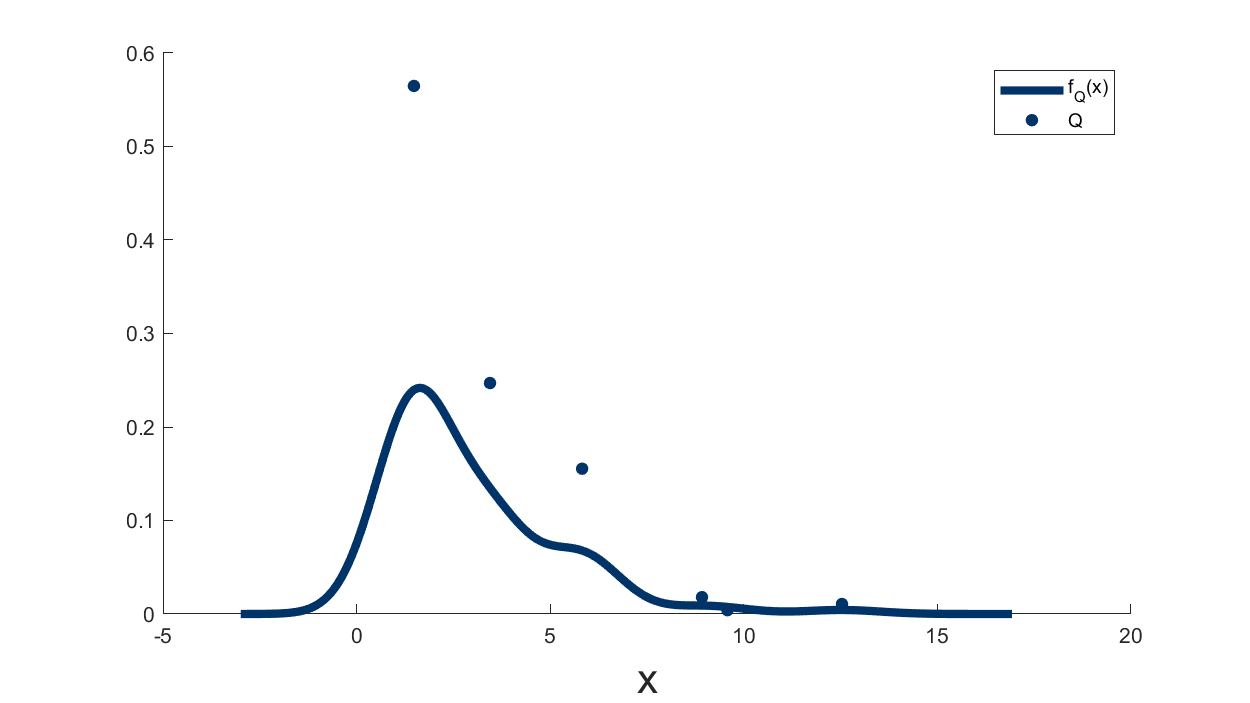
\includegraphics[width = \textwidth]{Figures/Mixtures/chi2_n500_motivation.png}
		\caption{A maximum likelihood location mixture of $n = 500$ points where the maximising mixing distribution, $Q$, has only 6 points of support.}
		\label{fig:chi2 n500 motivation}
	\end{figure}

	% While one can construct examples in which the mixing distribution that maximizes the likelihood has all $n$ points of support, in practise, 
	The size of the support of the $Q$ that maximizes \eqref{eq:loglikelihood} is the primary quantity of interest for this chapter. We define it as follows. Let $\mathcal{Q}_n$ be the set of all discrete probability distributions on $\mathbb{R}$ with no more than $n$ points of support. Let
	\begin{equation}
		\hat{Q}_{\vect{x},f} = \{Q \in \mathcal{Q}_n: l(Q;\vect{x}) \geq l(Q';\vect{x}), \forall Q' \in \mathcal{Q}_n\}
	\end{equation}
	be the set of all global maximizers of \eqref{eq:loglikelihood}. Then define
	\begin{equation}
		K_\vect{x} = K(\vect{x}; f) = \min\{m : \mathcal{Q}_m \cap \hat{Q}_{\vect{x},f} \neq \emptyset\}
		\label{eq:K_x definition}
	\end{equation}
	which counts the smallest number of probability masses needed to maximize the likelihood.


	There are a few considerations to be made here. The first is that there is not necessarily a unique mixing distribution that maximizes \eqref{eq:loglikelihood} and so we have defined the quantity of interest as the smallest number of points of support required for a maximizing distribution. However, in many cases, including when the component density is from the exponential family, we know that the maximizing mixing distribution is unique. This question of uniqueness was addressed by Lindsay in \cite{Lindsay1983-tf} and in \cite{Lindsay1983a-he} for continuous univariate component densities in the exponential family. A generalization of these results to discrete exponential families can be found in \cite{Lindsay1993-rj}.

	The second, is that our choice to consider only location mixtures is significant in that it guarantees that the likelihood is bounded so long as the component density is bounded. In general, this is not the case. Consider the likelihood function for a mixture of normals parametrized by both the mean and variance. We can create a mixture by placing equally weighted normals with very small variance at each $x_i$ in our sample. This corresponds to a mixing distribution $Q$ which places probability mass $1/n$ at points $(x_i, \sigma^2)$ for $i = 1, \dots, n$. As $\sigma^2$ approaches zero, the density at each $x_i$, $f_Q(x_i)$, increases without bound and so the likelihood is unbounded. There are a number of techniques that can be employed to ensure the likelihood is bounded such as restricting the parameter space appropriately or restricting the number of components to some number that grows slowly with $n$ (the sieve method \cite{Grenander1981-dy}).

	The third, is that we should be careful to make a distinction between calculating $K_\vect{x}$ and choosing an appropriate number of components for a mixture model. The former is simply a deterministic property of an optimization problem whereas the latter is an in-depth and difficult problem which involves consideration of properties such as consistency, and the use of techniques such as information criteria and likelihood ratio. This latter problem is discussed in \cite[Chapter 6]{McLachlan2004-ik}. In particular, if each $X_i$ comes from a distribution with density $g(x) = f_Q(x)$ (that is, $g(x)$ is a mixture density itself) then we may consider the `true' number of components and using certain penalised log likelihood criteria, such as the Akaike information criterion (AIC) \cite{Akaike1974-bl} or the Bayesian information criterion (BIC) \cite{Schwarz1978-ci}, does not underestimate this quantity asymptotically \cite{Leroux1992-ek}. This suggests that we should not expect $K_\vect{x}$ (which is defined from an unpenalised likelihood) to necessarily be reflective of the properties of $g(x)$.
 
	% Not necessarily unique Q
	% Location mixtures only (otherwise unbounded likelihood and use all n points)
	% Mention sieves
	% NOT about recovering the 'true' number of components - we are using mixtures as a density approximation tool and are interested in the property of this optimization.

	% A location mixture on $\mathbb{R}$ with mixing distribution $Q$ and component density $f(x)$ can be written as
	% \begin{equation}
	% 	f_Q(x) = \int_{-\infty}^\infty f(x-\theta) \intd Q(\theta).
	% \label{eq:mixtureint}
	% \end{equation}

	% Given a sample $\vect{x} = (x_1,\dots,x_n)$, we wish to find a distribution that maximizes the log likelihood	
	% \begin{equation}
	% 	L(Q;\vect{x}) = \sum_{i = 1}^n \log(f_Q(x_i)).
	% \label{eq:loglikelihood}
	% \end{equation}
	% Lindsay showed that under quite general conditions, such a maximizing distribution exists and has no more than $n$ points of support \cite{Lindsay1983-tf}. It is therefore common to use
	% \begin{equation}
	% 	f_{\vect{p},\vect{\theta}}(x) = \sum_{j = 1}^m p_j f(x - \theta_j)
	% \label{eq:mixturesum}
	% \end{equation}
	% instead of \eqref{eq:mixtureint} as our definition of a location mixture. We note that \eqref{eq:mixtureint} is equivalent to \eqref{eq:mixturesum} in the case where $Q$ is a discrete distribution which places probability masses of weight $p_j$ at locations $\theta_j$, for $j = 1,\dots,m$. The order of the $x_i$ does not matter and so we will assume without loss of generality that $x_1 \leq x_2 \leq \dots \leq x_n$ throughout.
	
	% In this paper we are primarily interested in the number of probability masses that are required in the maximizing mixture. We will call this quantity $K_{\vect{x}}$. It should be noted that there is not always a unique mixing distribution that maximizes \eqref{eq:loglikelihood}. However we can choose $K_{\vect{x}}$ to be the smallest number of probability masses that any of the maximizing distributions have.
\section{Summary of Lindsay}
\label{sec:summary of Lindsay}

[PROOF READING UP TO HERE]

	To obtain results concerning $K_\vect{x}$ we will make use of the geometric approach employed by Lindsay in \cite{Lindsay1983-tf} and \cite{Lindsay1983a-he} and summarized later in \cite[Chapter 5]{Lindsay1995-sq}. This section is dedicated to laying out the basics of this approach and summarising the results that are most relevant to our work. Here, we assume that the component densities, $f(\vect{x};\vect{\theta})$, are bounded, but we do not restrict ourselves to finite location mixtures on the real line.

	\subsection{The likelihood curve}
	The key to Lindsay's approach is to reformulate the problem from optimizing over all mixing distributions, to optimizing an appropriate objective function over a convex set in $\mathbb{R}^n$. For a component density $f$, mixing distribution $Q$, and sample $(x_1, \dots, x_n)$, define the \emph{likelihood vector}
	\begin{equation}
		\vect{\gamma}(Q;\vect{x}, f) = (\gamma_1, \dots, \gamma_n) = (f_Q(x_1), \dots, f_Q(x_n))
		\label{eq:likelihood vector}
	\end{equation}
	and the objective function
	\begin{equation}
		\mathcal{L}(\vect{\gamma}) = \sum_{i = 1}^n \ln(\gamma_i).
	\end{equation}
	For fixed $\vect{x}$ and $f$, let $\mathcal{M}$ be the set of all possible values of the likelihood vector as $Q$ varies over the set of mixing distributions.
	% Let 
	% \begin{equation}
	% 	\mathcal{M} = \{\vect{\gamma}(Q;\vect{x}, f): \text{$Q$ is a probability distribution}\}
	% \end{equation}
	% be the set of all possible values of the likelihood vector. 
	A maximizing mixing distribution may be found by first finding the $\hat{\vect{\gamma}} \in \mathcal{M}$ that maximizes $\mathcal{L}(\vect{\gamma})$ and then solving for $Q$ the $n$ equations that arise by considering each component of 
	\begin{equation}
		\vect{\gamma}(Q; \vect{x}, f) = \hat{\vect{\gamma}}.
	\end{equation}

	To show that $\mathcal{M}$ is a convex set, consider the \emph{unicomponent likelihood vector}
	\begin{equation}
		\vect{\gamma}(\vect{\theta}; \vect{x}, f) = (f_\vect{\theta}(x_1), \dots, f_\vect{\theta}(x_n))
	\end{equation}
	where $f_\vect{\theta}$ is the mixture density corresponding to the mixing distribution that places all its mass at $\vect{\theta}$, that is, 
	\begin{equation}
		f_\vect{\theta}(x) = f(x; \vect{\theta}).
	\end{equation}
	For any probability distribution, $Q$, the likelihood vector can be represented by
	\begin{equation}
		\vect{\gamma}(Q; \vect{x}, f) = \int \vect{\gamma}(\vect{\theta}; \vect{x}, f) \intd Q(\vect{\theta})
	\end{equation}
	which for a finite mixture $Q$, with weights $p_j$ assigned to parameters $\vect{\theta}_j$, can be written as
	\begin{equation}
		\vect{\gamma}(Q;\vect{x},f) = \sum_{j = 1}^m p_j \vect{\gamma}(\vect{\theta}_j; \vect{x}, f).
	\end{equation}
	
	This leads to an alternative characterisation of $\mathcal{M}$. Define the \emph{unicomponent likelihood curve}
	\begin{equation}
		\Gamma_{\vect{x}, f} = \{\vect{\gamma}(\vect{\theta}; \vect{x}, f) : \vect{\theta} \in \Omega\}.
	\end{equation}
	Then
	\begin{equation}
		\mathcal{M} = \conv(\Gamma_{\vect{x}, f}),
	\end{equation}
	where we use $\conv(A)$ to denote the convex hull of $A$. We now state the following Theorem taken directly from \cite[Theorem 18]{Lindsay1995-sq} which is a consequence of the convexity of $\mathcal{M}$, and the concavity of $\mathcal{L}(\vect{\gamma})$.

	\begin{theorem}[\cite{Lindsay1995-sq}]
		Suppose that $\Gamma_{\vect{x}, f}$ is closed and bounded and that $\mathcal{M}$ contains at least one point with positive likelihood. Then there exists a unique $\hat{\vect{\gamma}} \in \partial \mathcal{M}$, the boundary of $\mathcal{M}$, such that $\hat{\vect{\gamma}}$ maximizes $\mathcal{L}(\vect{\gamma})$ over $\mathcal{M}$.
		\label{thm: lindsay maximizing likelihood vector point}
	\end{theorem}

	In addition to this, in \cite[Theorem 21]{Lindsay1995-sq} is stated the following.
	\begin{theorem}[\cite{Lindsay1995-sq}]
		The solution $\hat{\vect{\gamma}}$ can be represented as $\vect{\gamma}(\hat{Q};\vect{x}, f)$, where $\hat{Q}$ has no more than $n$ points of support.
		\label{thm: lindsay no more than n points}
	\end{theorem}
	This gives us our first bound on $K_\vect{x}$: for component densities that produce a closed and bounded likelihood curve,
	\begin{equation}
		K_\vect{x} \leq n.
	\end{equation}

	\subsection{All points separated by \texorpdfstring{$\alpha$}{a}}
		Lindsay states that for normal mixtures with fixed variance, $\sigma^2$, ``one can construct sets of data for which the bound [$K_\vect{x} = n$] is attained simply by spreading the observations widely apart,'' \cite[Section 5.2]{Lindsay1995-sq}. Here we make this intuition concrete by saying how far apart we should spread our observations to ensure that the mixing distribution has $n$ separate components.

		% Consider the situation in which $|x_i - x_j| > \alpha$ for all $i\neq j$. Intuitively, we would expect that there is some $\alpha^*$ such that if $\alpha > \alpha^*$ then $\vect{x} \in C_n$.
		
		\begin{theorem}
			Let $\vect{x} = (x_1, \dots, x_n)$ be the sample for which we are finding a maximum likelihood location mixture using $f(x)$ as our component density. Let $f(x)$ be a unimodal density on $\mathbb{R}$, symmetric about $x = 0$, and such that the conditions of Theorem \ref{thm: lindsay maximizing likelihood vector point} hold. Let $\alpha > 0$ be such that
			\begin{equation}
				\frac{f(\alpha/2)}{f(0)} < \frac{1}{n}\left(\frac{n-1}{n}\right)^{n-1}.
				\label{eq:alpha condition}
			\end{equation}
			

			Then if for all $i\neq j$, $|x_i - x_j| > \alpha$ we must have $K_\vect{x} = n$.
		\end{theorem}
		\begin{proof}
			First consider constructing the maximum likelihood mixture density using no more than $n-1$ components. Let $\hat{f}_{n-1}$ be this maximum likelihood mixture density of $\vect{x}$ with no more than $n-1$ components and let $L_{n-1}$ be the corresponding likelihood. Let $\vect{\theta}$ and $\vect{p}$ be the locations and weights for the probability masses of $\hat{f}_{n-1}$. Since all the $x_i$ are separated by at least $\alpha$, there exists an $x_{i^*}$ such that $|x_{i^*} - \theta_j|>\frac{\alpha}{2}$ for all $j$. Hence
			\begin{equation}
				\hat{f}_{n-1}(x_{i^*}) < f(\alpha/2),
			\end{equation}
			and so
			\begin{equation}
				L_{n-1} < f(\alpha/2) \prod_{i\neq i^*} \hat{f}_{n-1}(x_{i}).	
			\end{equation}
						
			We will now construct a mixture density that has one more component that $\hat{f}_{n-1}$. We do this by scaling all the components of $\hat{f}_{n-1}$ by a factor of $\frac{n-1}{n}$ and introducing a new component with parameters $(\theta, p) = (x_{i^*},\frac{1}{n})$. Call this function $f^*_n$ and the corresponding likelihood $L_n$. At each $x_i \neq x_{i^*}$ the likelihood has decreased by $(n-1)/n$ and at $x_{i^*}$ the likelihood is at least $f(0)/n$. So
			\begin{equation}
				L_n > \frac{f(0)}{n} \left(\frac{n-1}{n}\right)^{n-1}\prod_{i\neq i^*} \hat{f}_{n-1}(x_i).	
			\end{equation}
			
			By \eqref{eq:alpha condition}, we get that $L_n > L_{n-1}$. Since the likelihood strictly increases when we allow an additional component, the maximum likelihood solution must have at least $n$ components. By Theorem \ref{thm: lindsay no more than n points}, the maximum likelihood solution cannot have any more than $n$ components and so $K_\vect{x} = n$.
		\end{proof}

	% \subsection{The likelihood curve}
	% 	In \cite{Lindsay1983-tf}, the problem of mixture likelihoods was looked at from a geometrical perspective. One key construction introduced by Lindsay was the \emph{likelihood curve},
	% 	\begin{equation}
	% 		\vect{\gamma}(\theta;\vect{x}) = (f(x_{1}-\theta),\dots,f(x_{n}-\theta))
	% 		\label{eq:Gamma}
	% 	\end{equation}
	% 	and it's trace,
	% 	\begin{equation}
	% 		\Gamma_{\vect{x}} = \{\vect{\gamma}(\theta;\vect{x})| \theta \in \mathbb{R}\}.
	% 	\end{equation}
	% 	A useful property of the likelihood curve is that any convex combination of elements from $\Gamma_{\vect{x}}$ can be written as
	% 	\begin{equation}
	% 		\vect{u}(\vect{p},\vect{\theta};\vect{x}) = (f_{\vect{p},\vect{\theta}}(x_{1}),\dots,f_{\vect{p},\vect{\theta}}(x_{n})) = \sum_{j = 1}^m p_j \vect{\gamma}(\theta_j;\vect{x}), \hspace{30pt} \sum_{j=1}^m p_j = 1
	% 		\label{eq:convexcombinationgamma}
	% 	\end{equation}
	% 	where $f_{\vect{p},\vect{\theta}}(x)$ is as defined in \eqref{eq:mixturesum}. The log likelihood of the corresponding distribution is simply the sum of the log of the components of $\vect{u}(\vect{p},\vect{\theta};\vect{x})$.
		
	% 	One of Lindsay's main results, which follows from this observation, was that if
	% 	\begin{equation}
	% 		\hat{\vect{u}} = \argmax_{\vect{u} \in \conv(\Gamma_{\vect{x}})} \sum_{i=1}^n \log(u_i)
	% 		\label{eq:optimalu}
	% 	\end{equation}
	% 	% where
	% 	% \begin{equation}
	% 	% 	U =  %\{\vect{u}(\vect{p},\vect{\theta};\vect{x}) |  \}
	% 	% \end{equation}
	% 	then we can write
	% 	\begin{equation}
	% 		\hat{\vect{u}} = \vect{u}(\vect{p},\vect{\theta};\vect{x})
	% 	\end{equation}
	% 	for some $\vect{p}$ and $\vect{\theta}$ whose dimension is no more than $n$. Furthermore, the corresponding distribution that places masses $p_j$ at locations $\theta_j$ maximizes \eqref{eq:loglikelihood}. There are some minor conditions on this result, but they will not cause any problems for our purposes and so will not be discussed (see \cite{Lindsay1983-tf} for details).
	\subsection{An example likelihood curve}
		\label{sec:mixturelikelihoods:example}
		In simple cases, we can plot the likelihood curve, $\Gamma_{\vect{x}, f}$, and objective function, $\mathcal{L}$, along with the maximizing point, $\hat{\vect{\gamma}}$. In particular, when $n = 2$, $\Gamma_{\vect{x}, f} \subset \mathbb{R}^2$ and if the component density is smoothly parametrized by a single parameter, then we can plot $\Gamma_{\vect{x}, f}$ by tracing out $\vect{\gamma}(\theta; \vect{x}, f)$ as we vary $\theta$.

		For example, suppose our sample is made up of two points, $\vect{x} = (x_1, x_2) = (1,2)$, and suppose our component density is normal with variance $\sigma_2 = 0.4^2$ and parametrized by $\theta$, that is,
		\begin{equation}
		f(x;\theta) = \frac{1}{0.4 \sqrt{2 \pi}} \exp\left(-\frac{(x-\theta)^2}{2\cdot 0.4^2}\right).
		\label{eq:example component density for likelihood curve}
		\end{equation}
		Then the corresponding likelihood curve can be traced out as we increase $\theta$ from $-\infty$ to $\infty$ as shown in Figure \ref{fig:TracingGamma}. 

		\begin{figure}[ht]
			\centering
			\begin{minipage}[b]{0.32\linewidth}
				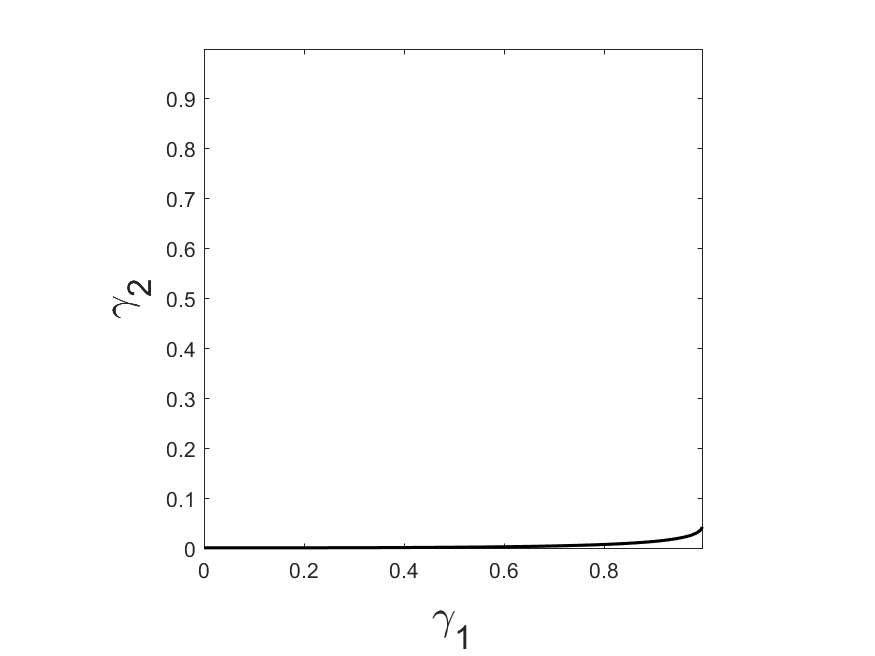
\includegraphics[width=\textwidth]{GammaTrace01}
			\end{minipage}
			\begin{minipage}[b]{0.32\linewidth}
				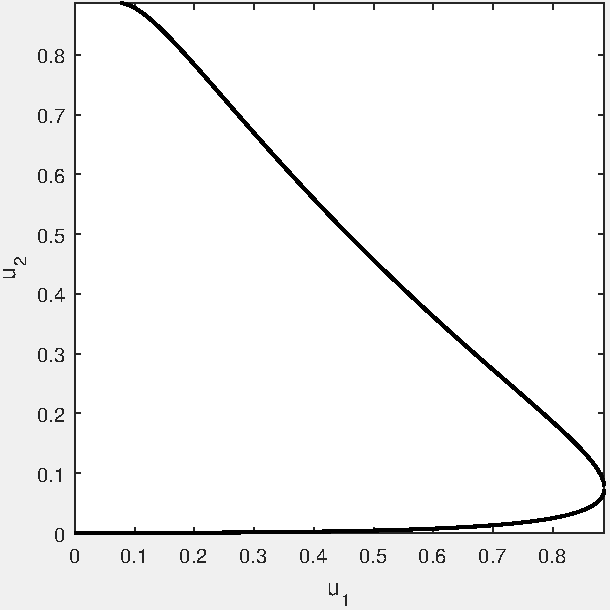
\includegraphics[width=\textwidth]{GammaTrace02}
			\end{minipage}
			\begin{minipage}[b]{0.32\linewidth}
				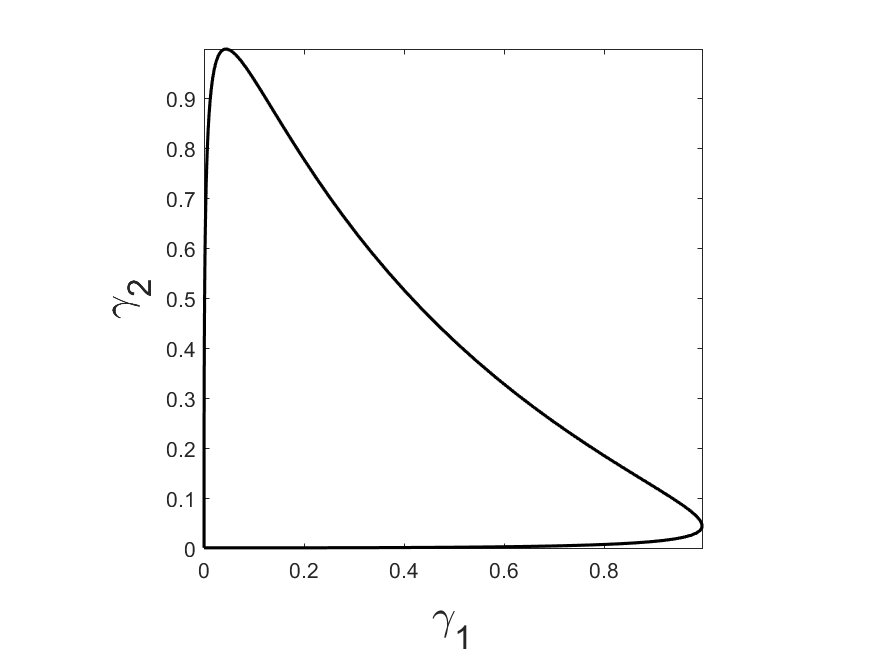
\includegraphics[width=\textwidth]{GammaTrace03}
			\end{minipage}
			\begin{minipage}[b]{0.32\linewidth}
				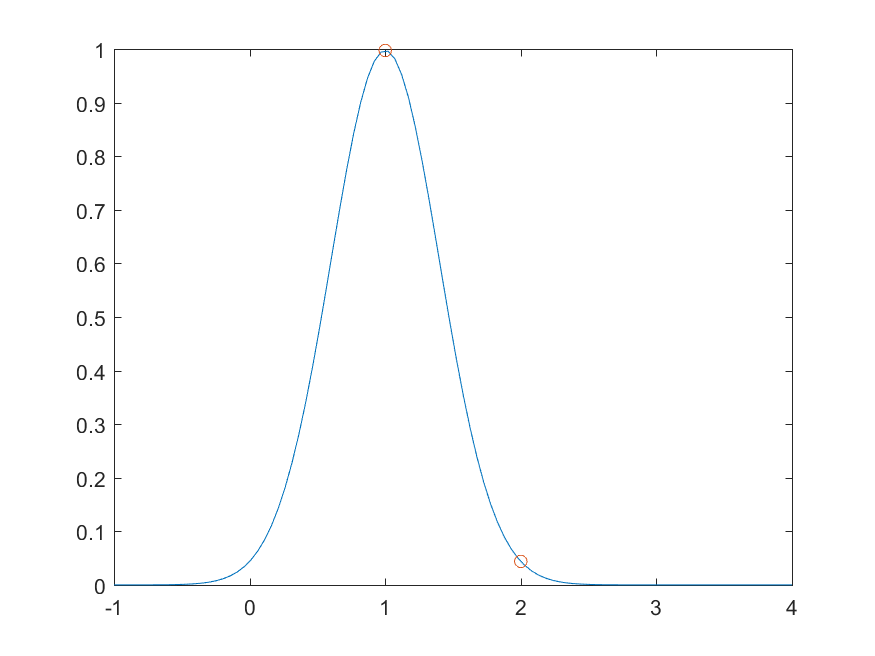
\includegraphics[width=\textwidth]{GammaTraceDensity01}
				\subcaption{$\theta = 1$}
			\end{minipage}
			\begin{minipage}[b]{0.32\linewidth}
				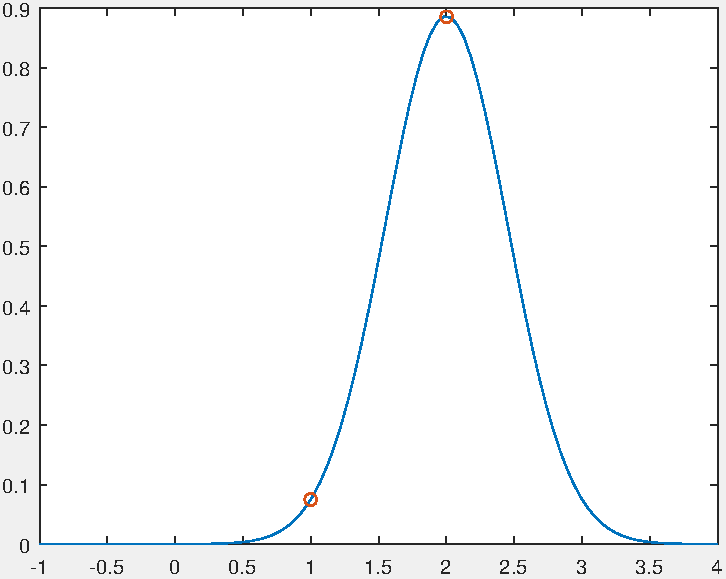
\includegraphics[width=\textwidth]{GammaTraceDensity02}
				\subcaption{$\theta = 2$}
			\end{minipage}
			\begin{minipage}[b]{0.32\linewidth}
				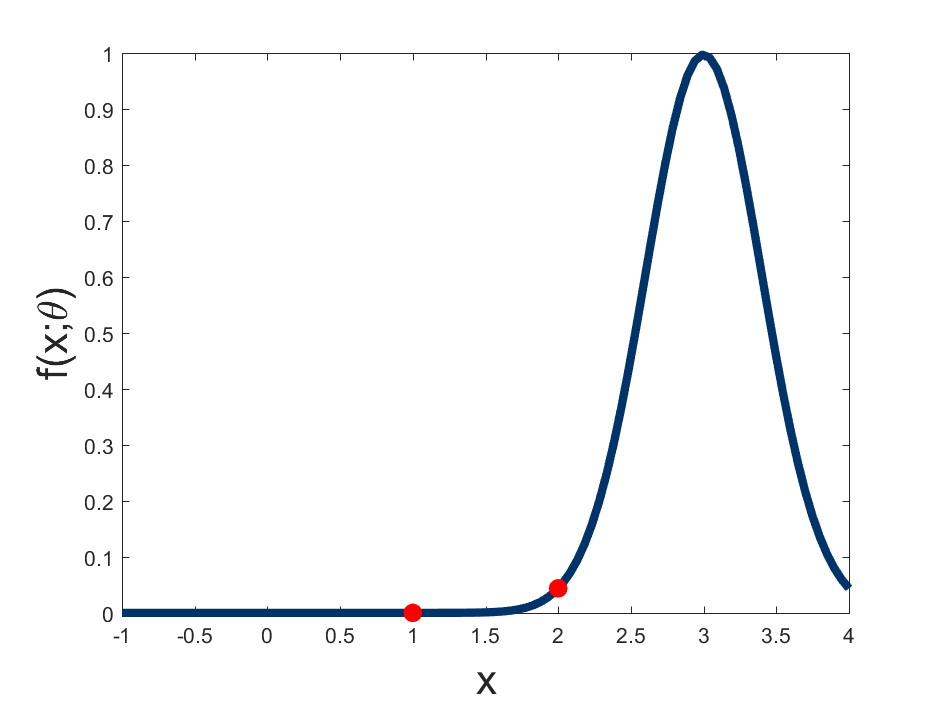
\includegraphics[width=\textwidth]{GammaTraceDensity03}
				\subcaption{$\theta = 3$}
			\end{minipage}
			\caption[A simple example of a likelihood curve.]{A simple example of a likelihood curve. The component density, $f(x;\theta)$, as defined in \eqref{eq:example component density for likelihood curve}, is shown in blue for $\theta = 1,2,$ and $3$. Each value of $\theta$ contributes a point to $\Gamma_{\vect{x}, f}$ whose coordinates are given by $(f(1;\theta),f(2;\theta))$ (represented by the heights of the red circles). As we increase $\theta$ from $-\infty$ to $\infty$ we trace out more of $\Gamma_{\vect{x}, f}$.}\label{fig:TracingGamma}
		\end{figure}

		
		The set of possible values of the likelihood vector, $\mathcal{M}$, is given by the convex hull of $\Gamma_{\vect{x}, f}$, the boundary of which is marked along with $\Gamma_{\vect{x}, f}$ in Figure \ref{fig:GammaSol:subfig:Gamma} and overlaid on a heat map of $\mathcal{L}(\vect{\gamma})$. The maximizing point, $\hat{\vect{\gamma}}$, is marked with a yellow dot and lies on the boundary of $\conv(\Gamma_{\vect{x}, f})$ as predicted by Theorem \ref{thm: lindsay maximizing likelihood vector point}. This point may be written as the convex combination of two points in $\Gamma_{\vect{x}, f}$,
		\begin{equation}
			\hat{\vect{\gamma}} = \sum_{j = 1}^2 p_j \vect{\gamma}(\theta_j;\vect{x}, f)
		\end{equation}
		and we represent the two points, $\vect{\gamma}(\theta_1;\vect{x}, f)$ and $\vect{\gamma}(\theta_2;\vect{x}, f)$ with magenta dots.

		The mixture $\hat{Q}$ that satisfies $\hat{\vect{\gamma}} = \vect{\gamma}(\hat{Q};\vect{x}, f)$ is the one that places masses $p_1$ and $p_2$ at locations $\theta_1$ and $\theta_2$ and it is plotted in Figure \ref{fig:GammaSol:subfig:Density} by two magenta points at $(\theta_1, p_1)$ and $(\theta_2, p_2)$ along with the overall mixture density $f_{\hat{Q}}(x)$.

		% The optimal point is on the boundary of $\conv(\Gamma)$ as expected and it can be written as the  $p_1 \vect{f}(\theta_1) + p_2 \vect{f}(\theta_2)$ (where $p_1 + p_2 =1 $). These two points correspond to the two probability masses in the maximizing mixture distribution shown in Figure \ref{fig:GammaSol:subfig:Density}. These masses are located at $\theta_1$ and $\theta_2$ with weights $p_1$ and $p_2$.

		%and so we will provide a slightly more general form of Theorem \ref{thm:LindsayGamma}.
		%\begin{theorem}
		%	Write $\vect{0}$ for the zero vector in $\mathbb{R}^n$. If $\Gamma \cup \{ \vect{0} \}$ is compact then there exists a unique point on the boundary of $\conv(\Gamma)$ which maximizes the likelihood. This point corresponds to a distribution $Q$ which maximizes the likelihood and that has no more than $n$ point masses.
		%\end{theorem}
		%\begin{proof}
		%	We need to show that $\vect{0}$ does not appear in the maximizing mixture. Clearly, $\vect{0}$ is not going to be a maximizing point.
		%\end{proof}

		% We trace the boundary of $\conv(\Gamma)$ in Figure \ref{fig:GammaSol} along with a heat map of the objective function \eqref{eq:transformedlikelihood}.

		\begin{figure}[ht]
			\centering
			\begin{minipage}{0.49\textwidth}
				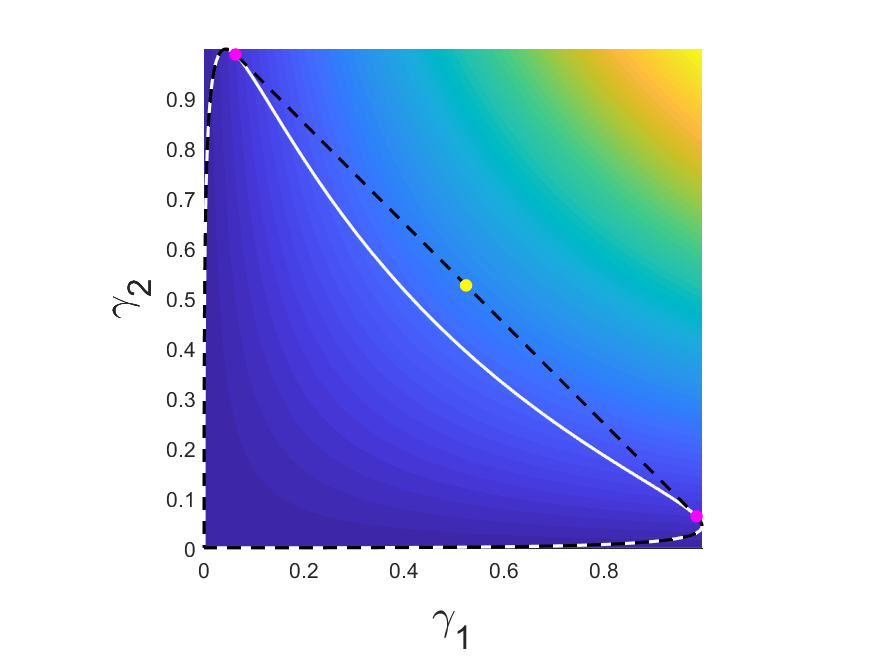
\includegraphics[width = \textwidth]{gamma_likelihood_heatmap}
				\subcaption{}\label{fig:GammaSol:subfig:Gamma}
			\end{minipage}
			\begin{minipage}{0.49\textwidth}
				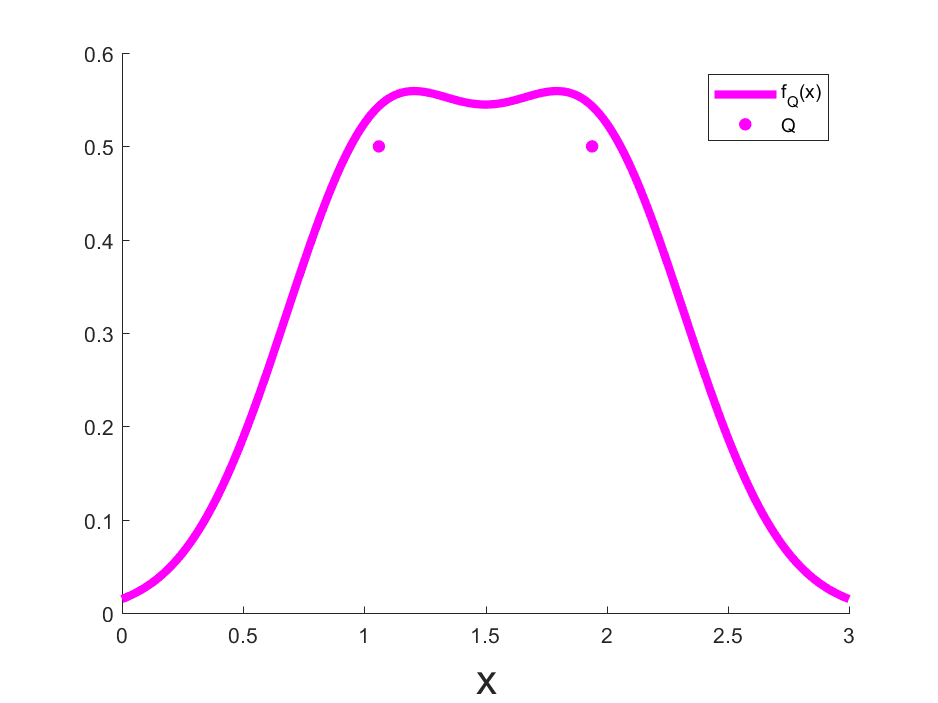
\includegraphics[width = \textwidth]{gamma_likelihood_heatmap_solution}
				\subcaption{}\label{fig:GammaSol:subfig:Density}
			\end{minipage}
			\caption[The geometric relationship between the likelihood curve (\subref{fig:GammaSol:subfig:Gamma}) and the maximizing mixture density (\subref{fig:GammaSol:subfig:Density}).]{The geometric relationship between the likelihood curve (\subref{fig:GammaSol:subfig:Gamma}) and the maximizing mixture density (\subref{fig:GammaSol:subfig:Density}). In (\subref{fig:GammaSol:subfig:Gamma}), the boundary of $\conv(\Gamma_{\vect{x}, f})$ is shown as a dashed black line, $\Gamma_{\vect{x}, f}$ is the white curve, the heat map  shows the objective function (likelihood increases from blue to yellow) and $\hat{\vect{\gamma}}$ is marked with a yellow dot. This point is a convex combination of the two magenta points. These two magenta points correspond to the two probability masses in the maximizing mixing distribution (\subref{fig:GammaSol:subfig:Density}).}
			\label{fig:GammaSol}
		\end{figure}

		\begin{remark}
			Note that in this example, while $\Gamma_{\vect{x}, f}$ is bounded, it is not closed (it does not contain the limit point $(0,0)$), counter to the requirements of Theorems \ref{thm: lindsay maximizing likelihood vector point} and \ref{thm: lindsay no more than n points}. In fact, any positive density whose support is the whole real line will not contain the limit point $\vect{0}$ (where $\vect{0}$ represents the zero vector in $\mathbb{R}^n$). However, since $\vect{0}$ is clearly not going to be a part of a maximizing mixture, we are safe to apply both theorems if $\Gamma \cup \{ \vect{0} \}$ is closed. A more detailed discussion concerning how to relax the requirement that the set $\Gamma_{\vect{x},f}$ be closed can be found in \cite[Section 5.2.2.]{Lindsay1995-sq}.
		\end{remark}

	\subsection{Gradient characterization}
	\label{sec: gradient characterization}
	Another important construction due to Lindsay is the gradient function
	\begin{equation}
		D_Q(\vect{\theta}; \vect{x}, f) = -n + \sum_{i = 1}^n \frac{f(x_i;\vect{\theta})}{f_Q(x_i)}.
		\label{eq:def gradient function}
	\end{equation}
	For each value of $\theta \in \Omega$, this is the derivative of $l(Q;\vect{x},f)$ as we move along the path parametrized by
	\begin{equation}
		(1 - p)Q + p\Delta_\vect{\theta}
	\end{equation}
	evaluated at $p = 0$ and where $\Delta_\vect{\theta}$ is a degenerate distribution that places all of its mass at $\vect{\theta}$. In \cite[Theorem 4.1]{Lindsay1983-tf}, Lindsay showed we can characterise the maximizing mixture by three equivalent conditions. The statement of the Theorem here is taken from \cite[Theorem 19]{Lindsay1995-sq}.

	\begin{theorem}[\cite{Lindsay1995-sq}]
	\label{thm:Lindsay three statements that characterise maximizing mixture}
		The following three statements are equivalent:
		\begin{enumerate}
			\item $\hat{Q}$ maximizes $l(Q;\vect{x},f)$.
			\item $\hat{Q}$ minimizes $\sup_\vect{\theta} D_Q(\vect{\theta};\vect{x}, f)$.
			\item $\sup_\vect{\theta} D_{\hat{Q}}(\vect{\theta};\vect{x}, f) = 0$.
			\label{item:supremum of gradient is zero}
		\end{enumerate}
	\end{theorem}

	The intuition here is that $D_Q(\vect{\theta}; \vect{x}, f)$ measures the change in likelihood as we move a little bit of mass from each of the points of support of $Q$ to a point at $\vect{\theta}$. If a mixing distribution $\hat{Q}$ maximizes the likelihood, then this change in likelihood should never be positive and if we are not at the maximizing distribution $\hat{Q}$, then there should be some $\vect{\theta}$ to which we can move some mass to increase the likelihood.

	% [BLAHBLAH]

	Also contained in \cite[Theorem 4.1]{Lindsay1983-tf} was the following result concerning the locations of the support points of $\hat{Q}$. The statement here is taken from \cite[Theorem 20]{Lindsay1995-sq}.

	\begin{theorem}[\cite{Lindsay1995-sq}]
		\label{thm: Lindsay support is zeros of gradient}
		The support of any maximum likelihood estimator $\hat{Q}$ lies in the set 
		\begin{equation}
			\left\{\vect{\theta} : D_{\hat{Q}}(\vect{\theta};\vect{x},f) = 0 \right\}.
			\label{eq:set D_Q = 0}
		\end{equation}
	\end{theorem}

	Theorems \ref{thm:Lindsay three statements that characterise maximizing mixture} and \ref{thm: Lindsay support is zeros of gradient} indicate that each support point of $\hat{Q}$ is a local maximum of $D_{\hat{Q}}(\vect{\theta}; \vect{x}, f)$. So if $f$ is parametrized by a single parameter $\theta$ and $D_Q(\theta;\vect{x},f)$ is twice differentiable in $\theta$, then each support point $\theta^*$ of the maximizing mixture distribution, $\hat{Q}$, satisfies
	\begin{align}
		D_{\hat{Q}}(\theta^*;\vect{x}, f) &= 0, 
		\label{eq:Deq1}\\
		D'_{\hat{Q}}(\theta^*;\vect{x}, f) &= 0, 
		\label{eq:Deq2}\\
		D''_{\hat{Q}}(\theta^*;\vect{x}, f) &\leq 0,
		\label{eq:Deq3}
	\end{align}
	so long as $\theta^*$ is not on the boundary of the parameter space. A typical example of this is shown in Figure \ref{fig:D_Q example}. In this figure we observe that $D_Q(\theta)$ has a local maximum at every point where $Q$ places a probability mass. Since $D_Q(\theta) \leq 0$ for all $\theta \in \mathbb{R}$, we know that $Q$ is the maximum likelihood mixing distribution. In Section \ref{sec:KKT conditions} we will show how to obtain equations \eqref{eq:Deq1} and \eqref{eq:Deq2} using a different method to Lindsay that does not involve the gradient function.

	% [EXAMPLE]

	\begin{figure}[ht]
		\begin{subfigure}[t]{0.49\textwidth}
			\centering
			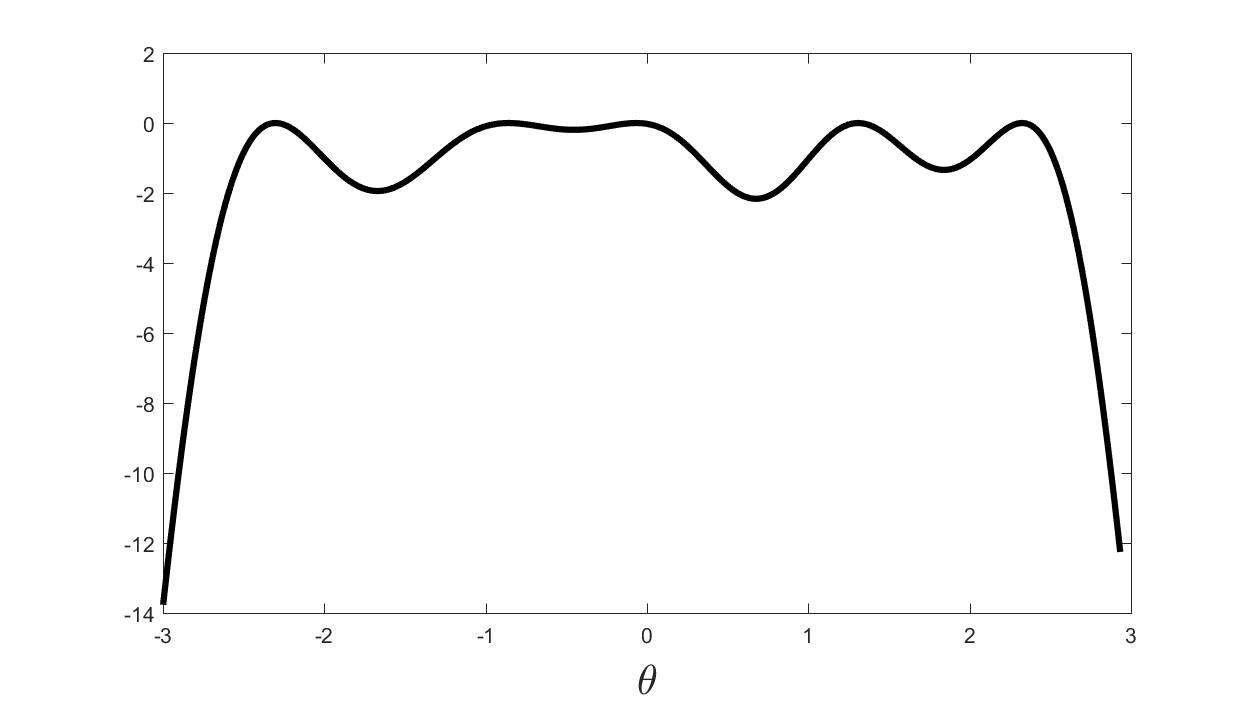
\includegraphics[width = \textwidth]{Figures/Mixtures/D_Q_example.png}
			\caption{}\label{subfig:D_Q}
		\end{subfigure}
		\begin{subfigure}[t]{0.49\textwidth}
			\centering
			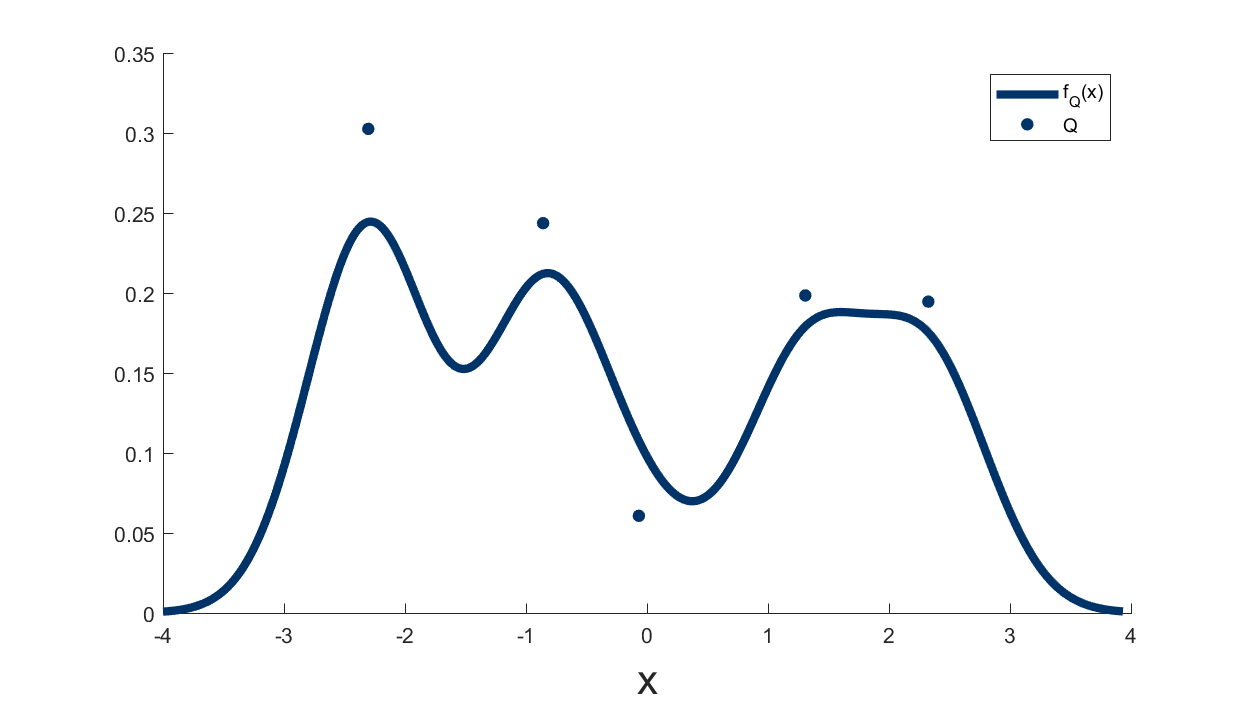
\includegraphics[width = \textwidth]{Figures/Mixtures/D_Q_example_mixture.png}
			\caption{}\label{subfig:D_Qmixture}
		\end{subfigure}
		\caption[The gradient function and its associated mixing distribution and mixture.]{The gradient function, $D_{\hat{Q}}$, (\subref{subfig:D_Q}) and its associated mixing distribution, $Q$, and mixture, $f_Q$, (\subref{subfig:D_Qmixture}). In this example $f$ is normal with variance $1/4$ and $\vect{x}$ is made up of $n = 50$ points distributed uniformly but randomly along $[-3, 3]$.}
		\label{fig:D_Q example}
	\end{figure}

	\subsubsection{Support Hyperplane}
	\label{sec: support hyperplane}
	There is a geometric interpretation to these theorems that ties in with the likelihood curve interpretation given above. For any given mixing distribution $Q$, define the \emph{inverse likelihood vector} $\vect{\lambda}(Q;\vect{x},f) = (1/f_Q(x_1),\dots, 1/f_Q(x_n))$ and the hyperplane
	\begin{equation}
		\mathcal{H}_{Q} = \{\vect{z} : \langle \vect{\lambda}(Q;\vect{x},f), \vect{z}\rangle = n\},
	\end{equation}
	which contains the usual likelihood vector, $\vect{\gamma}(Q;\vect{x}, f)$. We may write the gradient function as
	\begin{equation}
		D(Q;\vect{x},f) = \langle \vect{\lambda}(Q;\vect{x},f), \vect{\gamma}(\vect{\theta};\vect{x},f)\rangle - n.
	\end{equation}
	If $\hat{Q}$ maximizes $l(Q;\vect{x},f)$ then by statement \ref{item:supremum of gradient is zero} of Theorem \ref{thm:Lindsay three statements that characterise maximizing mixture}, 
	\begin{equation}
		\langle \vect{\lambda}(\hat{Q};\vect{x},f), \vect{\gamma}(\vect{\theta};\vect{x},f) \rangle \leq n
	\end{equation}
	for all $\vect{\theta} \in \Omega$. This means that $\mathcal{M} = \conv(\Gamma_{\vect{x},f})$ lies entirely on one side of $\mathcal{H}$ and Theorem \ref{thm: Lindsay support is zeros of gradient} tell us that if $\vect{\theta}$ is in the support of $\hat{Q}$, then 
	\begin{equation}
		\langle \vect{\lambda}(\hat{Q};\vect{x},f), \vect{\gamma}(\vect{\theta};\vect{x},f) \rangle = n
	\end{equation}
	and so $\vect{\gamma}(\vect{\theta};\vect{x},f) \in \mathcal{H}$. Thus we can gain information about the number of support points of $\hat{Q}$ by finding the number of points at which $\Gamma_{\vect{x},f}$ touches $\mathcal{H}_{\hat{Q}}$. As an example, consider Figure \ref{fig:cauchy support hyperplane}. Here we observe the likelihood curve for a Cauchy density and $n = 2$ observations. The support line containing $\hat{\vect{\gamma}}$ has two points of contact with $\Gamma_{\vect{x}, f}$ which correspond to the two points of support of the maximum likelihood mixture $\hat{Q}$. In our experience it is fairly typical for every contact point of $\Gamma_{\vect{x}, f}$ with $\mathcal{H}_{\hat{Q}}$ (or equivalently, every point in \eqref{eq:set D_Q = 0}) to correspond to a support point of $\hat{Q}$. However, this is not always the case. In Figure \ref{fig:triangle support hyperplane} we have shown the likelihood curve for a symmetric triangular density and $n =2$ observations. We observe that $\mathcal{H}_{\hat{Q}}$ touches $\Gamma_{\vect{x}, f}$ at an infinite number of points along a line segment. The interpretation is that there are an infinite number of distinct mixtures which achieve the maximum likelihood, each with support points corresponding to various locations along that line segment.

	\begin{figure}
		\centering
		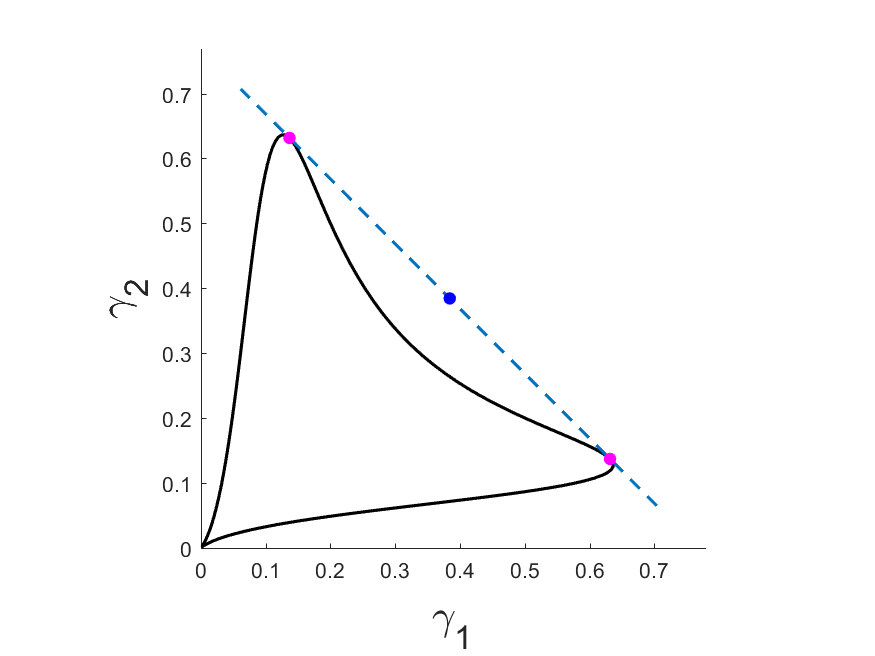
\includegraphics[width = 0.9\textwidth]{Figures/Mixtures/cauchy_support_hyperplane.png}
		\caption{The likelihood curve, $\Gamma_{\vect{x}, f}$, (solid line) along with the support hyperplane, $\mathcal{H}_{\hat{Q}}$, (dashed line) that contains $\hat{\vect{\gamma}}$ (blue point), and the points of contact with $\Gamma_{\vect{x}, f}$ (magenta points). In this example $\vect{x} = (1,2)$ and $f$ is a Cauchy density with scale parameter $1/2$.}
		\label{fig:cauchy support hyperplane}
	\end{figure}

	\begin{figure}
		\centering
		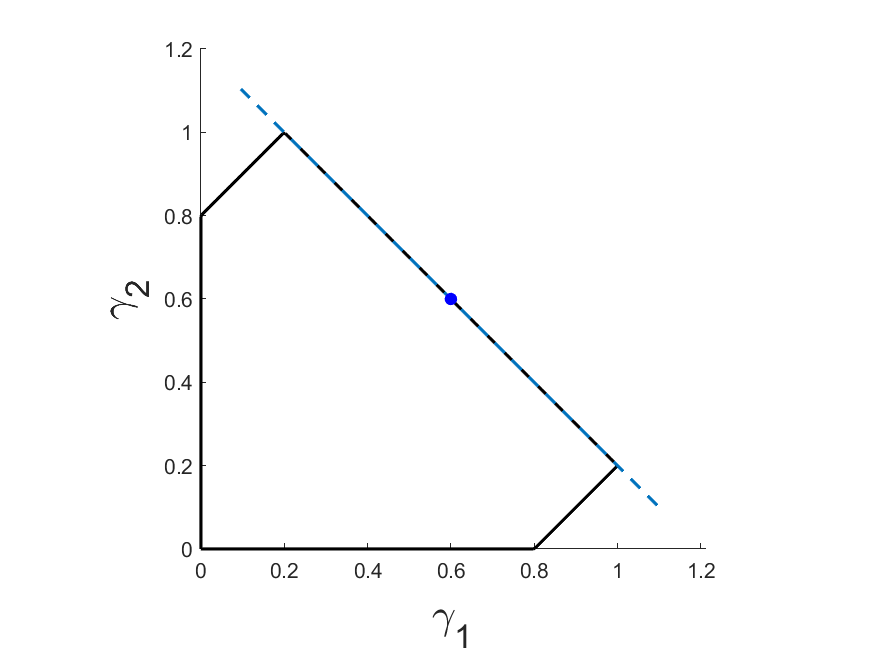
\includegraphics[width = 0.9\textwidth]{Figures/Mixtures/triangle_density_gamma.png}
		\caption{The likelihood curve, $\Gamma_{\vect{x}, f}$, (solid line) along with the support hyperplane, $\mathcal{H}_{\hat{Q}}$, (dashed line) that contains $\hat{\vect{\gamma}}$ (blue point). In this example $\vect{x} = (0,0.4)$ and $f$ is a symmetric triangular density with width $1/2$.}
		\label{fig:triangle support hyperplane}
	\end{figure}

	\subsection{KKT conditions}
	\label{sec:KKT conditions}
	We will now point out that the gradient function conditions in \eqref{eq:Deq1} and \eqref{eq:Deq2} can be obtained using the Karush-Kuhn-Tucker (KKT) conditions \cite{Kuhn1951-ih} \cite{Karush2014-vk} for the following optimisation problem. Suppose that we restrict our mixture to have no more than $m$ components. Then given a component density $f$, and data $\vect{x}$, the problem of finding the maximum likelihood location mixture can be written as the following non-linear optimization problem.

	Find $\vect{\theta}$ and $\vect{p}$ that maximize
	\begin{equation}
		l_m(\vect{\theta},\vect{p};\vect{x}) = \sum_{i=1}^n \log \left[\sum_{j=1}^m p_j f(x_i - \theta_j) \right]
		\label{eq:l_m}
	\end{equation}
	subject to 
	\begin{align}
		&\theta_j -\theta_{j+1} \leq 0, &&j=1,\dots,m-1
		\label{eq:constraintheta}\\
		&-p_j \leq 0, &&j=1,\dots,m
		\label{eq:constrainpj}\\
		&\sum_{j=1}^m p_j = 1.
		\label{eq:constrainpjequal}
	\end{align}

	Constraints \eqref{eq:constrainpj} and \eqref{eq:constrainpjequal} ensure that the mixture is valid. We also include \eqref{eq:constraintheta} so that any mixture which can be written with fewer than $m$ components appears on the boundary of the feasible space (we will either have some $p_j = 0$ or some $\theta_j = \theta_{j+1}$). Conversely, any point at which we have equality in any of the constraints in \eqref{eq:constraintheta} or \eqref{eq:constrainpj}, can be written with fewer than $m$ components. Hence, a necessary condition for $K_\vect{x} = m$ is that any maximizing point of \eqref{eq:l_m} must also satisfy strict inequalities in \eqref{eq:constraintheta} and \eqref{eq:constrainpj}.

	Introduce Lagrange multipliers $\lambda$, $\vect{\mu}$, $\vect{\nu}$ and form the Lagrangian
	\begin{equation}
		\mathcal{L}(\vect{\theta},\vect{p},\lambda,\vect{\mu},\vect{\nu}) = l_m(\vect{\theta},\vect{p};\vect{x}) - \lambda\left(1 - \sum_{j=1}^m p_j\right) - \sum_{j=1}^m \mu_j p_j + \sum_{j=1}^{m-1} \nu_j \left(\theta_j - \theta_{j+1}\right).
		\label{eq:kkt lagrangian}
	\end{equation}
	The KKT conditions tell us that at a local maximum the equations
	\begin{align}
		&\frac{\partial}{\partial \theta_1} l_m(\vect{\theta},\vect{p};\vect{x}) = \nu_1 \label{eq:KKTtheta1}\\ 
		&\frac{\partial}{\partial \theta_j} l_m(\vect{\theta},\vect{p};\vect{x}) = \nu_j - \nu_{j-1}, &&j=2,\dots,m-1 \label{eq:KKTtheta}\\ 
		&\frac{\partial}{\partial \theta_m} l_m(\vect{\theta},\vect{p};\vect{x}) = -\nu_{m-1} \label{eq:KKTthetam}\\ 
		&\frac{\partial}{\partial p_j} l_m(\vect{\theta},\vect{p};\vect{x}) = \lambda - \mu_j && j = 1,\dots,m. \label{eq:KKTlambda}
	\end{align}
	must be satisfied along with the constraints in \eqref{eq:constraintheta}, \eqref{eq:constrainpj}, \eqref{eq:constrainpjequal}, and the additional constraints
	\begin{align}
		&\vect{\mu},\vect{\nu} \geq 0,\\
		&\mu_j p_j = 0, &&j=1,\dots,m \label{eq:mujpjconstraint}\\
		&\nu_j (\theta_j - \theta_{j+1}) = 0, &&j=1,\dots,m-1.
		\label{eq:nujthetajconstraint}
	\end{align}

	Multiplying both sides of \eqref{eq:KKTlambda} by $p_j$ (recall \eqref{eq:mujpjconstraint}) and summing over $j$ we get that
	\begin{equation}
		\lambda = \sum_{j = 1}^m p_j \frac{\partial}{\partial p_j} l_m(\vect{\theta},\vect{p};\vect{x}).
	\end{equation}
	From \eqref{eq:l_m},
	\begin{align}
		\lambda &= \sum_{j = 1}^m p_j \frac{\partial}{\partial p_j} \left( \sum_{i=1}^n \log \left[\sum_{k=1}^m p_k f(x_i - \theta_k) \right] \right)\\
			&= \sum_{j = 1}^m p_j \sum_{i=1}^n \frac{f(x_i - \theta_j)}{\sum_{k=1}^m p_k f(x_i - \theta_k)}\\
			&= \sum_{i=1}^n \sum_{j=1}^m  \frac{p_j f(x_i - \theta_j)}{\sum_{k=1}^m p_k f(x_i - \theta_k)}\\
			&= n.
	\end{align}

	If we additionally require that the solution uses all $m$ components, then we must have that $p_j > 0$, and $\theta_j - \theta_{j+1} < 0$ for all $j$. Constraints \eqref{eq:mujpjconstraint} and \eqref{eq:nujthetajconstraint} then require $\mu_j = 0$ and $\nu_j = 0$ for all $j$. This gives us necessary conditions for $\hat{Q} = (\vect{\theta}, \vect{p})$ to be an $m$ point maximizing mixture,
	\begin{align}
		&-n + \frac{\partial}{\partial p_j} l_m(\vect{\theta},\vect{p};\vect{x}) = 0, && j = 1,\dots,m\\
		&\frac{\partial}{\partial \theta_j} l_m(\vect{\theta},\vect{p};\vect{x}) = 0, && j = 1,\dots, m.
	\end{align}
	Substituting in $l_m$ from \eqref{eq:l_m} we obtain
	\begin{align}
		&-n + \sum_{i=1}^n \frac{f(x_i - \theta_j)}{f_{\hat{Q}}(x_i)} = D_{\hat{Q}}(\theta_j;\vect{x}, f) =  0 && j = 1, \dots, m \label{eq:KKT Deq1}\\
		&\sum_{i=1}^n \frac{-p_jf'(x_i - \theta_j)}{f_{\hat{Q}}(x_i)} = p_j D_{\hat{Q}}'(\theta_j;\vect{x}, f) = 0 && j = 1, \dots, m
		\label{eq:KKT Deq2}
	\end{align}
	which are equivalent to \eqref{eq:Deq1} and \eqref{eq:Deq2} respectively.

	% [KEEP THIS SECOND ORDER STUFF IN?]
	% [COMMENT ON LINDSAY THM 7.1]
	% [CHECK FOR MISTAKES IN MY WORK AND LINDSAY'S]
	% [IF NO MISTAKES SAY "NOT WHAT WE GOT" (if they are comparable)]

	The second order conditions are slightly more complex. In the context of our problem they state \cite[Proposition 3.3.1]{Bertsekas1995-mh} that a necessary condition for the point $(\vect{\theta}, \vect{p}, \lambda, \vect{\mu}, \vect{\nu})$ to be a local maximum is that,
	% \begin{equation}
	% 	y' 
	% 	\begin{bmatrix}
	% 		\frac{\partial^2}{\partial \theta_1^2} & \frac{\partial^2}{\partial \theta_1 \theta_2} & \dots & \frac{\partial^2}{\partial \theta_1 p_1} & \dots\\
	% 		\frac{\partial^2}{\partial \theta_2 \theta_1} & \frac{\partial^2}{\partial \theta_1^2} & \dots & \vdots  & \dots\\
	% 		\vdots & & \ddots & &\\
	% 		\vdots & & & \frac{\partial^2}{\partial p_1^2} &\\
	% 		\vdots & & \ddots & &
	% 	\end{bmatrix} y \geq 0.
	% \end{equation}
	\begin{equation}
		\vect{y}' \nabla^2_{\vect{\theta}, \vect{p}} \mathcal{L}(\vect{\theta}, \vect{p}, \lambda, \vect{\mu}, \vect{\nu}) \vect{y} \leq 0
		\label{eq:KKT second order}
	\end{equation}
	for all $\vect{y} \in \mathbb{R}^{2m}$ such that
	\begin{equation}
		\nabla h(\vect{\theta}, \vect{p})' \vect{y} = 0.
	\end{equation}
	where
	\begin{equation}
		h(\vect{\theta}, \vect{p}) = 1 - \sum_{j = 1}^m p_j.
	\end{equation}
	Since 
	\begin{equation}
		\nabla h(\vect{\theta}, \vect{p}) = (0, \dots, 0, -1, \dots, -1),
	\end{equation}{}
	equation \eqref{eq:KKT second order} must be satisfied in particular for $\vect{y}$ with components $y_k = 1$ for some $k \leq m$ and $y_i  = 0$ for all $i \neq k$. This gives us that necessary conditions for $\hat{Q}$ to be an $m$ point maximum are that
	\begin{align}
		\frac{\partial^2}{\partial \theta_j} \mathcal{L}(\vect{\theta}, \vect{p}, \lambda, \vect{\mu}, \vect{\nu}) &\leq 0, && j = 1, \dots, m.
	\end{align}
	Recalling \eqref{eq:kkt lagrangian} and \eqref{eq:l_m}, we get that
	\begin{align}
		\frac{\partial^2}{\partial \theta_j} \mathcal{L}(\vect{\theta}, \vect{p}, \lambda, \vect{\mu}, \vect{\nu}) &= \sum_{i = 1}^n \frac{p_j f''(x_i - \theta_j)}{\sum_{k = 1}^m p_k f(x_i - \theta_k)} - \sum_{i = 1}^n \left(\frac{p_j f'(x_i - \theta_j)}{\sum_{k = 1}^m p_k f(x_i - \theta_k)}\right)^2 \\
		&= p_j D_Q''(\theta_j;\vect{x}, f) - \sum_{i = 1}^n \left(\frac{p_j f'(x_i - \theta_j)}{\sum_{k = 1}^m p_k f(x_i - \theta_k)}\right)^2 \\
		&\leq 0.
	\end{align}
	Overall, we have that at every support point, $\theta^*$, of an $m$-point maximizing mixture, $Q$, we must have that
	\begin{equation}
		D_Q''(\theta^*;\vect{x},f) \leq p^* \sum_{i = 1}^n \left(\frac{f'(x_i - \theta_j)}{\sum_{k = 1}^m p_k f(x_i - \theta_k)}\right)^2.
		\label{eq: our second order KKT condition}
	\end{equation}
	This is a weaker condition than that in \eqref{eq:Deq3}. We were unable to obtain an equivalent condition to \eqref{eq:Deq3} using the above method. This is somewhat expected as we have restricted our mixture to have no more than $m$ components, whereas the condition in \eqref{eq:Deq3} relates to the global maximizing mixture distribution.

	We note that Lindsay presented a similar result in \cite[Theorem 7.1]{Lindsay1983-tf} and \cite[Theorem 24]{Lindsay1995-sq} which concerned maximum likelihood estimators with a fixed number of components, $m$. Below we rewrite this statement in the context of location mixtures.
	\begin{claim}[\cite{Lindsay1995-sq}, Theorem 24]
	\label{thm:Lindsay m-point conditions}
		Let $\tilde{Q}_m$ be a mixing distribution that maximizes the $m$ component location mixture likelihood, and let $\theta^*$ be a support point of $\tilde{Q}_m$. If the gradient function is twice differentiable at $\theta^*$, then:
		\begin{align}
			D_{\tilde{Q}_m}(\theta^*; \vect{x}, f) &= 0,\\
			D_{\tilde{Q}_m}'(\theta^*; \vect{x}, f) &= 0,\\
			D_{\tilde{Q}_m}''(\theta^*; \vect{x}, f) &\leq \sum_{i = 1}^n \left(\frac{f(x_i - \theta^*)}{\sum_{k = 1}^m p_k f(x_i - \theta_k)}\right)^2.
			\label{eq:Lindsay m-point Deq 3}
		\end{align}
	\end{claim}

	Equations \eqref{eq: our second order KKT condition} and \eqref{eq:Lindsay m-point Deq 3} appear similar in form but are not equivalent. Lindsay did not provide a proof for his statement but asserted that Claim \ref{thm:Lindsay m-point conditions} can be proved in a straightforward way using the likelihood equations and the formula for the gradient. We are unable to replicate his result, and instead present a counter-example to Claim \ref{thm:Lindsay m-point conditions}.

	Let our component density $f$ be normal with unit variance, and let $\vect{x} = (-2,2)$. Consider the mixing distribution, $\tilde{Q}_1$, that maximizes the 1 component location mixture likelihood. It has one support point, $\theta_1$. The gradient function for this distribution is given by
	\begin{equation}
		D_{\tilde{Q}_1}(\theta;\vect{x}, f) = -n + \sum_{i = 1}^2 \frac{f(x_i - \theta)}{f(x_i - \theta_1)}
	\end{equation}
	with derivatives
	\begin{equation}
		D_{\tilde{Q}_1}'(\theta;\vect{x}, f) = \sum_{i = 1}^2 \frac{-f'(x_i - \theta)}{f(x_i - \theta_1)} = \sum_{i = 1}^2 \frac{(x_i - \theta) f(x_i - \theta)}{f(x_i - \theta_1)}
	\end{equation}
	and
	\begin{equation}
		D_{\tilde{Q}_1}''(\theta;\vect{x}, f) = \sum_{i = 1}^2 \frac{f''(x_i - \theta)}{f(x_i - \theta_1)} = \sum_{i = 1}^2 \frac{((x_i - \theta)^2 - 1)f(x_i - \theta)}{f(x_i - \theta_1)},
	\end{equation}
	where
	\begin{equation}
		f(x) = \frac{1}{\sqrt{2 \pi}} \exp\left(-\frac{x^2}{2}\right).
	\end{equation}
	By \eqref{eq:KKT Deq2}, we must have that $D'_{\tilde{Q}_1}(\theta_1;\vect{x}, f) = (x_1 - \theta_1) + (x_2 - \theta_1) = 0$ and so $\theta_1 = 0$. Then it is simple to calculate
	\begin{equation}
		D_{\tilde{Q}_1}''(\theta_1;\vect{x}, f) = 6
	\end{equation}
	and
	\begin{equation}
		\sum_{i = 1}^n \left(\frac{f(x_i - \theta_1)}{\sum_{k = 1}^m p_k f(x_i - \theta_k)}\right)^2 = 2.
	\end{equation}
	Clearly \eqref{eq:Lindsay m-point Deq 3} does not hold. 

	By way of comparison, 
	\begin{equation}
		p_1 \sum_{i = 1}^n \left(\frac{f'(x_i - \theta_1)}{\sum_{k = 1}^m p_k f(x_i - \theta_k)}\right)^2 = \sum_{i = 1}^2 x_i^2 = 8,
	\end{equation}
	verifying that \eqref{eq: our second order KKT condition} holds for this example.


	\subsection{Additional results on \texorpdfstring{$K_\vect{x}$}{Kx}}

	Theorem \ref{thm: lindsay no more than n points} bounds $K_\vect{x}$ by $n$. To get tighter bounds on $K_\vect{x}$, we must make some assumptions about the form of the component densities, or the structure of $\vect{x}$.

	In \cite{Lindsay1983a-he}, Lindsay looked at the special case of  component densities in the exponential family. He related the behaviour of certain polynomials to the location of the support points of the maximizing mixture. A consequence of this was a sufficient condition for the maximizing mixture to have exactly one point of support. We restate part of this theorem here.

	\begin{theorem}[Theorem 4.1, \cite{Lindsay1983a-he}]
	\label{thm:exponential family k=1 bound}
		Let $f_\theta$ belong to the exponential class of densities and be parametrized by its mean value $\theta$. Let $\vect{x} = (x_1, \dots, x_n)$, $x_1 \leq \dots \leq x_n$, be the sample for which we are finding the maximum likelihood mixture of $f_\theta$. Define the function
		\begin{equation}
			M(\theta) = (x_1 - \theta)(x_n - \theta) + \var_\theta(X).
		\end{equation}
		If $M(\theta)$ is strictly positive on $[x_1, x_n]$, then the maximimum likelihood mixing distribution, $\hat{Q}$, has exactly one point of support located at $\theta = \bar{x}$.
	\end{theorem}

	The above is a sufficient condition for $K_\vect{x} = 1$. However, Linsday also showed that in the case of two observations ($n=2$), one could easily visualise the likelihood curve for a location mixture of normals and observe that the above sufficient condition also seems to be necessary for a normal density. 
	% \subsection{The likelihood curve when \texorpdfstring{$n = 2$}{n = 2}}
		% The shape of $\Gamma_\vect{x}$ can provide us with some insight into the behaviour of $K_\vect{x}$. 

	We illustrate this in Figure \ref{fig:Gammaexample} by giving some examples of $\Gamma_\vect{x}$ for $n=2$ using a normal component density with variance $\sigma^2 = 1$. 
	\begin{figure}[ht]
		\begin{subfigure}[t]{0.32\textwidth}
			\centering
			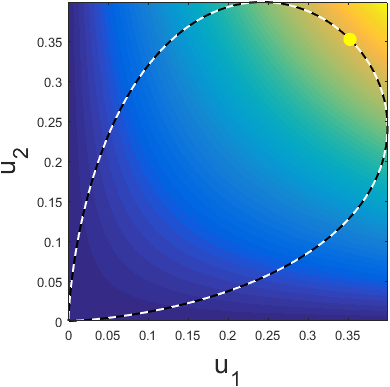
\includegraphics[width = \textwidth]{Sigma1x1_0-x2_1}
			\caption{$\vect{x} = (0,1)$} \label{subfig:gammaexamplea}
		\end{subfigure}
		\begin{subfigure}[t]{0.32\textwidth}
			\centering
			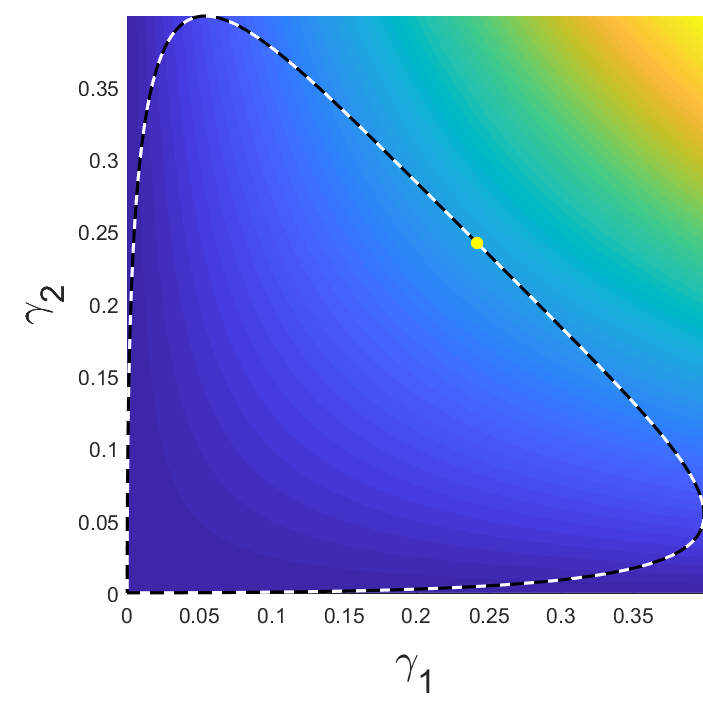
\includegraphics[width = \textwidth]{Sigma1x1_0-x2_2}
			\caption{$\vect{x} = (0,2)$} \label{subfig:gammaexampleb}
		\end{subfigure}
		\begin{subfigure}[t]{0.32\textwidth}
			\centering
			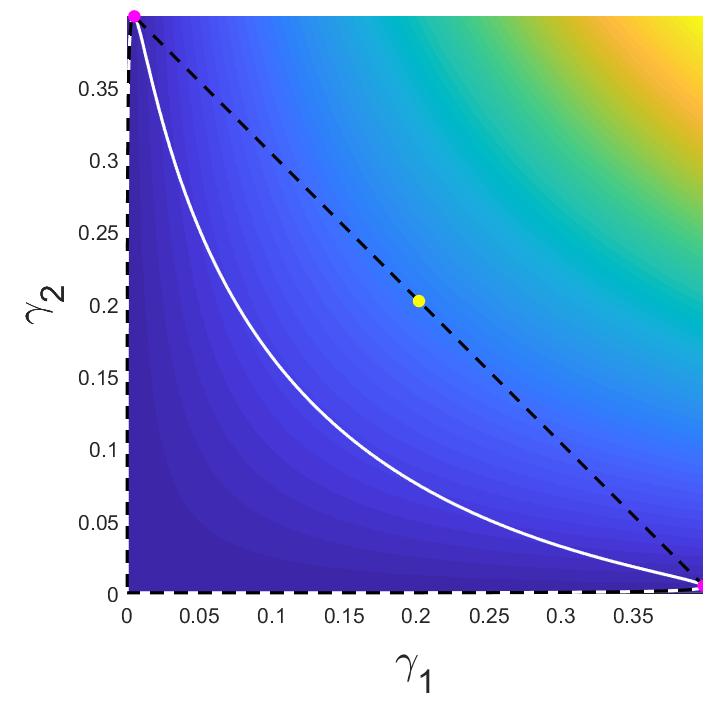
\includegraphics[width = \textwidth]{Sigma1x1_0-x2_3}
			\caption{$\vect{x} = (0,3)$} \label{subfig:gammaexamplec}
		\end{subfigure}
		\caption[The curve $\Gamma_\vect{x}$ for three different $\vect{x}$ along with the boundary of $\conv(\Gamma_\vect{x})$ for a normal component density with unit variance.]{The curve $\Gamma_\vect{x}$ for three different $\vect{x}$ along with the boundary of $\conv(\Gamma_\vect{x})$ for a normal component density with unit variance. The objective function, $\mathcal{L}(\vect{\gamma})$, is represented as a heat map. The optimal point $\hat{\vect{\gamma}}$ is shown in yellow, and where applicable, the points $\vect{\gamma}(\theta_j)$ that make up $\hat{\vect{\gamma}}$ are shown in magenta.}
		\label{fig:Gammaexample}
	\end{figure}
%
	In particular, we note that the distance between $x_1$ and $x_2$ has a strong effect on the shape of $\Gamma_\vect{x}$. In Figure \ref{subfig:gammaexamplea}, the points are distance 1 apart and $\Gamma_\vect{x}$ is the boundary of $\conv(\Gamma_\vect{x})$. In this case, it is clear that $K_\vect{x} = 1$. In Figure \ref{subfig:gammaexamplec}, the points are distance 3 apart and the optimal point no longer lies on $\Gamma_\vect{x}$. This results in the maximum likelihood mixing distribution needing two points of support and so $K_\vect{x} = 2$. The boundary case, where $\Gamma_\vect{x}$ goes from being a convex curve to having the indentation shown in Figure \ref{subfig:gammaexamplec}, is shown in Figure \ref{subfig:gammaexampleb}. This corresponds to the maximum separation the two points can have while keeping $M(\theta)$ non-negative on $[x_1, x_n]$.


	% Obtaining results about where these boundaries lie is very difficult in higher dimensions. In \cite{Lindsay1983a-he}, Lindsay used the sign of the curvature of $\vect{\gamma}(\theta;\vect{x})$ to obtain results for $n=2$ when the component density is in the exponential family.
	Lindsay stated that "these results were very difficult to obtain in higher dimensions, and hard to generalize outside the exponential family" \cite{Lindsay1995-sq}. Some generalizations to the results in \cite{Lindsay1983a-he} were presented in \cite{Lindsay1993-rj}. This paper gave improved bounds on $K_\vect{x}$ for discrete component densities.

	In Section \ref{sec:mixture results} we will present a necessary and sufficient condition for $K_\vect{x} = 1$ in the case of two observations for a certain class of densities that include the normal density, as well as other densities outside the exponential family. We will also present a necessary condition for $K_\vect{x} = m$, $m = 1, \dots, n$, for normal densities in the case of $n$ observations.

	% [WE USE UNIMODALITY TO BE ABLE TO JUST LOOK AT CURVATURE ALONG INTERVAL]

	% [FOLLOWING IS NOTES FOR MYSELF]

	% Exponential family \cite{Lindsay1983a-he}, more general results including this one and others in \cite{Lindsay1993-rj}. In particular, $n/2$ for discrete densities. May want to cite \cite{Seregin2010-xe} since it has some very limited results on the support. Read \cite{Zhang2008-wn} for more citations.
	

	% \subsection{Directional Derivative}
	% 	One of the tools introduced in \cite{Lindsay1983-tf} was the function
	% 	\begin{equation}
	% 		D(\theta;\vect{p},\vect{\theta},\vect{x}) = -n + \sum_{i=1}^n \frac{f(x_i - \theta)}{\sum_{j=1}^m p_j f(x_i - \theta_j)}.
	% 	\end{equation}

	% 	Lindsay showed that if $\hat{\vect{\theta}}$ and $\hat{\vect{p}}$ form a maximum likelihood location mixture of $f$ for $\vect{x}$ then (under appropriate differentiability assumuptions) the function $D$ satisfies the following:
	% 	% \begin{align}
	% 	% 	D(\theta_k;\hat{\vect{p}},\hat{\vect{\theta}},\vect{x}) &= 0, && k = 1,\dots,m,
	% 	% 	\label{eq:Deq1}\\
	% 	% 	D'(\theta_k;\hat{\vect{p}},\hat{\vect{\theta}},\vect{x}) &= 0, && k = 1,\dots,m,
	% 	% 	\label{eq:Deq2}\\
	% 	% 	D''(\theta_k;\hat{\vect{p}},\hat{\vect{\theta}},\vect{x}) &\leq 0, && k = 1,\dots,m.
	% 	% 	\label{eq:Deq3}
	% 	% \end{align}
	% 	These three constraints restrict what a potential maximum likelihood solution can look like.
	% 	HOW DID LINDSAY USE THEM VS US?


\section{Empirical Results}
\label{sec:empirical results}
	In this section we explore $K_\vect{x}$ through empirical results and figures. Throughout this section, and for the remainder of this chapter, we will consider only location mixtures (see \eqref{eq:location mixture}). All component densities will be unimodal, with a mode at $x = 0$. We list in Table \ref{tab:component densities} the component densities that we will use.

	\begin{table}[ht]
	\centering
		\begin{tabular}{l | c}
			Density & $f(x) = $\\
			\hline
			normal with fixed variance $\sigma^2$ & $\frac{1}{\sigma \sqrt{2 \pi}} \exp\left(-\frac{x^2}{2\sigma^2}\right) $\\
			Cauchy with fixed scale $\gamma$ & $\frac{1}{\pi \gamma + \pi x^2/\gamma}$
		\end{tabular}	
		\caption{List of component densities we consider.}
		\label{tab:component densities}
	\end{table}
	

	\subsection{Method}
	There are two parts to determining $K_\vect{x}$ empirically. The first part is to find the maximum likelihood mixture, $\hat{Q}$, or at least a good approximation $Q^*$. Given $\vect{x} \in \mathbb{R}^n$, we use a general purpose nonlinear programming solver (the MATLAB function \emph{fmincon}) to find the maximum likelihood mixture. We can test that we have indeed reached the global maximum through the use of the derivative function conditions given in Theorem \ref{thm:Lindsay three statements that characterise maximizing mixture}. If the mixture that is returned by our general solver does not satisfy these conditions then we may use another method, such as the vertex direction method (VDM) or the vertex exchange method (VEM), which is guaranteed to converge to the global maximum but converges slowly (see \cite{Bohning1995-di} for a review of different methods). We note that the actual method used is not important so long as the final result satisfies the derivative conditions. In practice, when $n$ is small, a general purpose solver is sufficient, fast, and simple to implement, and we rarely need to use a secondary method.

	The second part is to determine the number of points of support of $Q^*$. We initiate our general purpose solver with a mixture distribution that has more points of support than is needed. Under the optimization, this collapses down to the distribution $Q^*$ which may assign zero weight to some masses, and may concentrate multiple masses on the one point of support. We may simplify such a distribution by removing all masses with zero weight, and by combining all masses which share a point of support into one mass which takes the combined weight of the constituent masses (see Figure \ref{fig:collapsing distribution}). A naive approach would be to take the number of probability masses in this simplified distribution as the value for $K_\vect{x}$.

	\begin{figure}
		\centering
		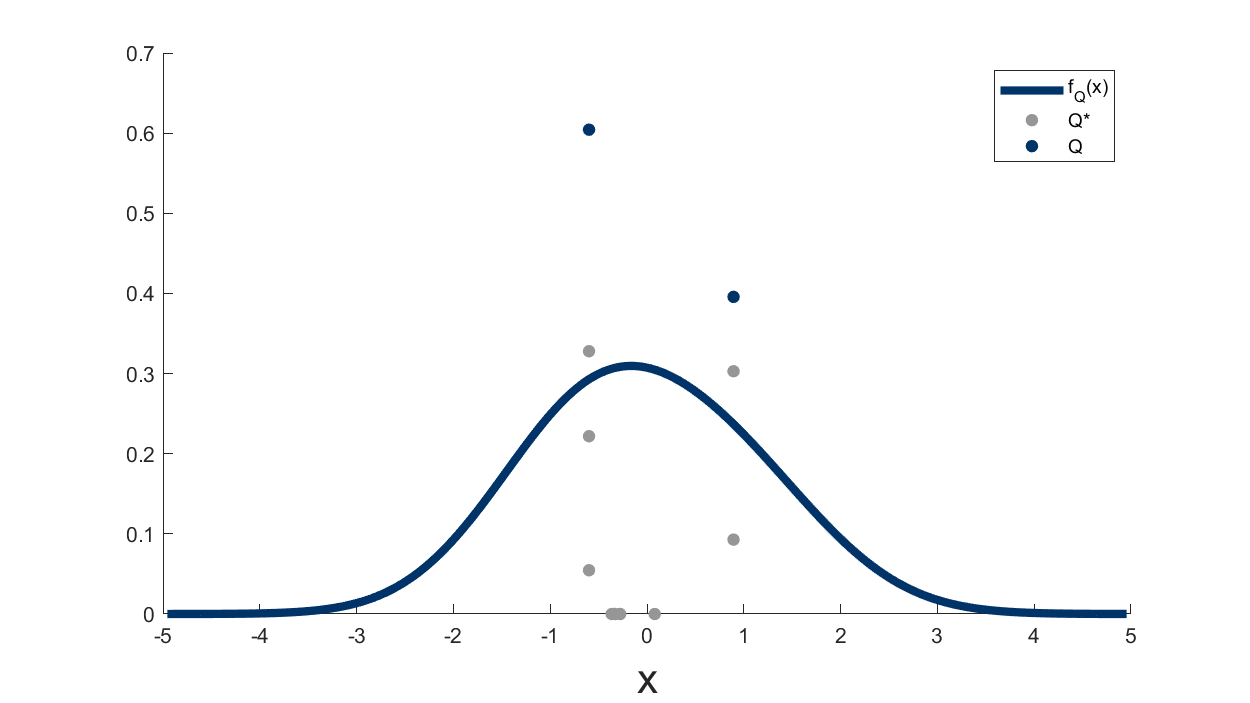
\includegraphics[width = \textwidth]{Figures/Mixtures/collapsing_distribution.png}
		\caption[The unsimplified mixing distribution $Q^*$ that results from using more points of support than required when finding our maximizing mixture, as well as the equivalent simplified distribution, $Q$, and the resulting mixture density, $f_Q(x)$.]{The unsimplified mixing distribution $Q^*$ that results from using more points of support than required when finding our maximizing mixture, as well as the equivalent simplified distribution, $Q$, and the resulting mixture density, $f_Q(x)$. Each probability mass with support $\theta$ and weight $p$ is represented by a point at $(\theta, p)$. In this example $\vect{x}$ is made up of $n = 50$ independent points distributed uniformly but randomly on the interval $[-2,-2]$, and $f$ is normal with unit variance.}
		\label{fig:collapsing distribution}
	\end{figure}

	However, there are some problems with this approach. In practice, we do not remove masses with exactly zero weight, but rather remove masses with weight $p_j < \epsilon$ for some small $\epsilon > 0$. Similarly, we merge masses $i$ and $j$ with support $|\theta_j - \theta_i| < \delta$ for some small $\delta > 0$. It may be that the true maximum likelihood mixture does contain components that have either very small weight, or are located very close to other masses. In this scenario, we would produce a value for $K_\vect{x}$ that is too small.

	Instead, we propose the following. From Theorem \ref{thm: Lindsay support is zeros of gradient}, each point of support, $\hat{\theta}_j$ of the maximizing mixture distribution $\hat{Q}$ is a local maximum of $D_{\hat{Q}}(\theta;\vect{x}, f)$ with $D_{\hat{Q}}(\theta_j;\vect{x},f) = 0$. So, given the mixing distribution $Q^*$ that results from our optimization, we take $K_\vect{x}$ to be the number of local maxima in $D_{Q^*}(\theta;\vect{x}, f)$ that take maximum value close to $0$. Note that $D_{\hat{Q}}(\theta_j; \vect{x}, f) = 0$ does not guarantee that $\theta_j$ is a support point of $\hat{Q}$ and so it is possible that this method produces a value for $K_\vect{x}$ that is too large. However, apart from some deliberately constructed scenarios, in our experience $D_{\hat{Q}}(\theta;\vect{x}, f)$ is typically zero only at the support points of $\hat{Q}$.

	% [WHEN IS SUPPORT ALWAYS EQUAL TO SET OF D(THETA) = 0?]

	% [EXTEND AS REQUIRED]
	% \subsection{Motivating Example?}

	\subsection{Flag graphs}
	\label{sec: flag graphs}
	When is $n$ is very small, we can plot $K_\vect{x}$ as a function of $\vect{x}$. For example, we may take $\vect{x} = (x_1, x_2)$ across a grid of values and colour each point $\vect{x}$ according to the value of $K_\vect{x}$. We have done this in Figure \ref{fig:normal_flag_graph_n2} for a normal component density with fixed variance $\sigma^2 = 1$. We observe a band in which $K_\vect{x} = 1$ and outside of which $K_\vect{x} = 2$.

	\begin{figure}
		\centering
		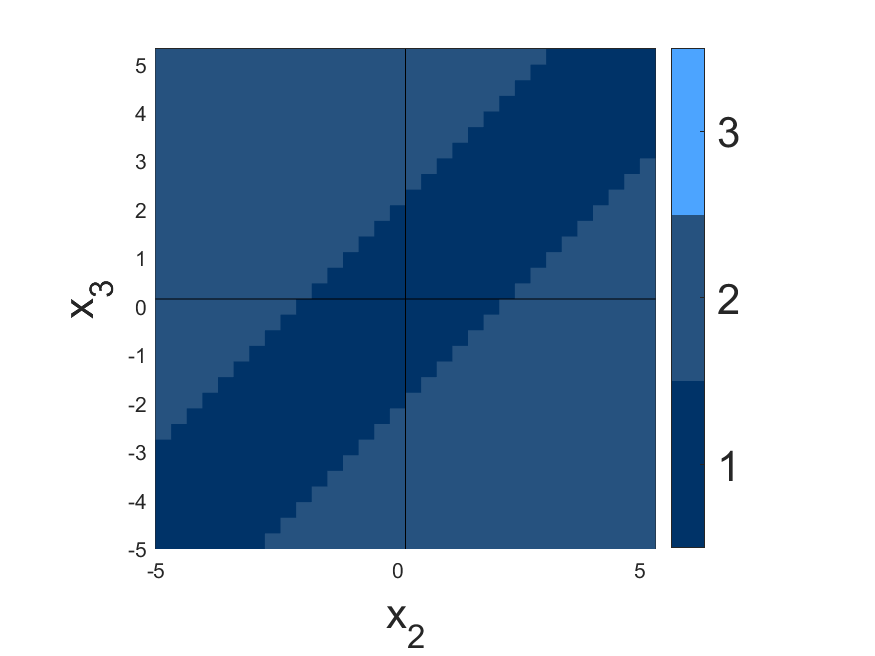
\includegraphics[width = 0.9\textwidth]{Figures/Mixtures/normal_flag_graph_n2.png}
		\caption{$K_\vect{x}$ as a function of $\vect{x} = (x_1, x_2)$, for a normal component density with fixed variance $\sigma^2 = 1$.}
		\label{fig:normal_flag_graph_n2}
	\end{figure}

	However, there is some redundancy in this plot which arises because we are using location mixtures. When using a location mixture, if the maximizing mixing distribution for $\vect{x}$ places weights $p_j$ at locations $\theta_j$, then a maximizing mixing distribution for $\vect{x} + (c, \dots, c)$ for some constant $c \in \mathbb{R}$ is simply the distribution that places weights $p_j$ at locations $\theta_j + c$. That is, shifting $\vect{x}$ by $c$ results in the maximizing mixture also shifting by $c$. A consequence of this fact is that $K_\vect{x}$ is invariant under translations of the form $\vect{x} \mapsto \vect{x} + (c, \dots, c)$.

	This suggests increasing $n$ to $3$, and fixing one of the $x_i$ while letting the other two vary. We do this by taking $\vect{x} = (0, x_2, x_3)$ with $x_2$ and $x_3$ varying across an evenly spaced grid. We do this for both a normal component density with variance $\sigma^2 = 1$ (Figure \ref{fig:normal_flag_graph}) and a Cauchy density with scale $\gamma = \sqrt{3}$ (Figure \ref{fig:cauchy_flag_graph}). We have chosen the scale of the Cauchy distribution so that it has inflection points in the same places as the normal density, namely at $x = \pm 1$. This decision is made in light of Theorem \ref{thm:n=2 inflection result} which says that for $n = 2$ and for certain component densities $f$, $K_\vect{x}$ can be determined by comparing $|x_1 - x_2|$ and the distance between the inflection points of $f$. It seems reasonable to expect that the choice of scale that makes the $n = 2$ figures identical is a good choice for comparing the effects of choosing different component densities in the $n = 3$ case.

	% One point that we wish to emphasize is that, given a component density $f$, $K$ is a function of $\vect{x}$ only. We can visualise this for small values of $n$. In Figure \ref{fig:normal_flag_graph}, we empirically found the MLE for $\vect{x} = (0,x_2,x_3)$ and recorded the number of probability masses in the maximizing mixture. We took values for $x_2$ and $x_3$ from an evenly spaced grid with $-6\leq x_2,x_3\leq 6$. We fixed $x_1 = 0$ since the shape of the maximum likelihood mixture (and therefore $K_{\vect{x}}$) depends only on the relative location of the $x_i$, not their absolute location.
	
	% \begin{figure}
	% 	\centering
	% 	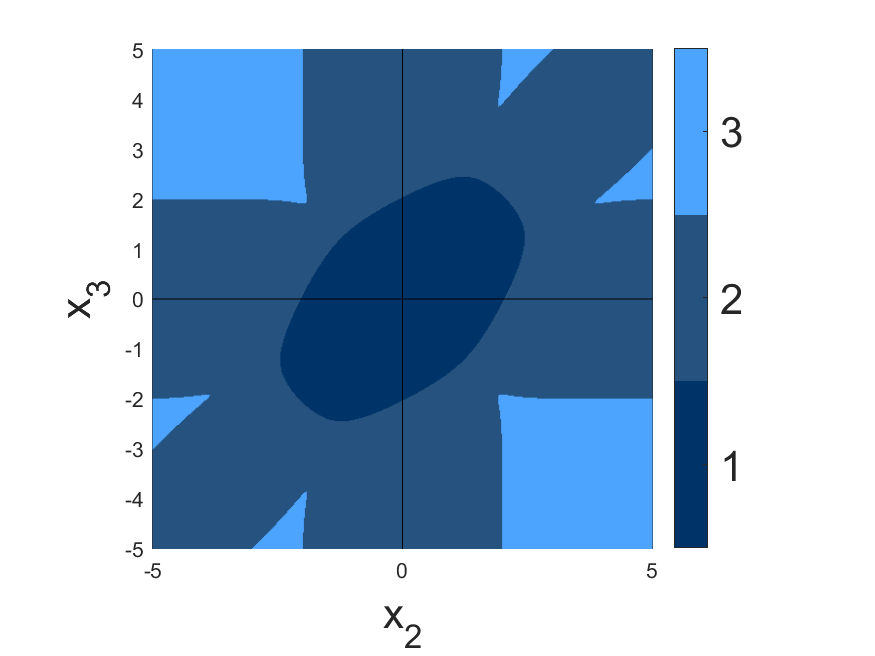
\includegraphics[width=0.9\textwidth]{normal_flag_graph.png}
	% 	\caption{$K_\vect{x}$ as a function of $\vect{x} = (0, x_2, x_3)$ for a normal component density with fixed variance $\sigma^2 = 1$.}\label{fig:normal_flag_graph}
	% \end{figure}

	% \begin{figure}
	% 	\centering
	% 	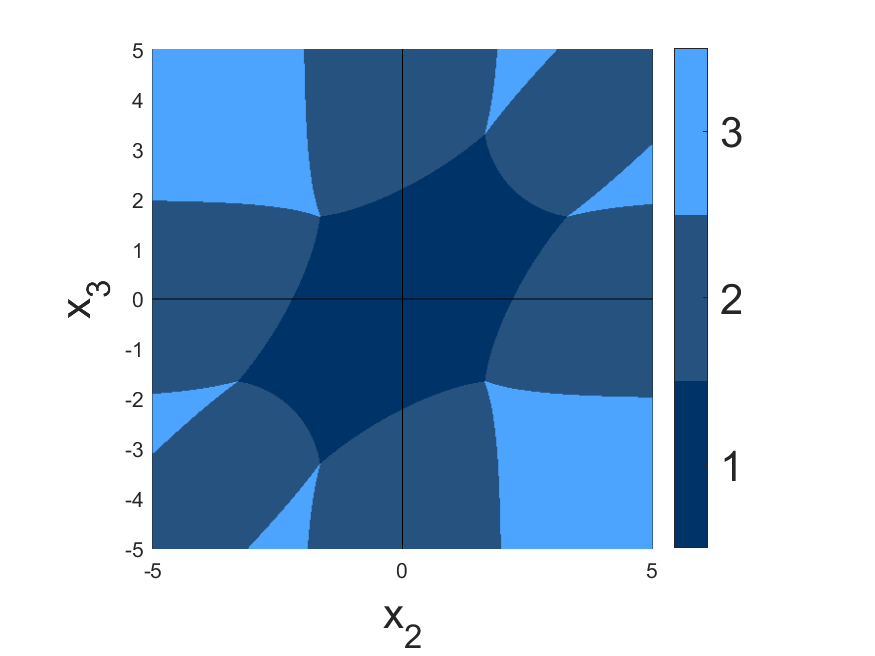
\includegraphics[width=0.9\textwidth]{cauchy_flag_graph.png}
	% 	\caption{$K_\vect{x}$ as a function of $\vect{x} = (0, x_2, x_3)$ for a Cauchy component density with fixed scale $\gamma = \sqrt{3}$.}
	% 	\label{fig:cauchy_flag_graph}
	% \end{figure}

	\begin{figure}[ht]
	\centering
		\begin{subfigure}[t]{0.49\textwidth}
			\centering
			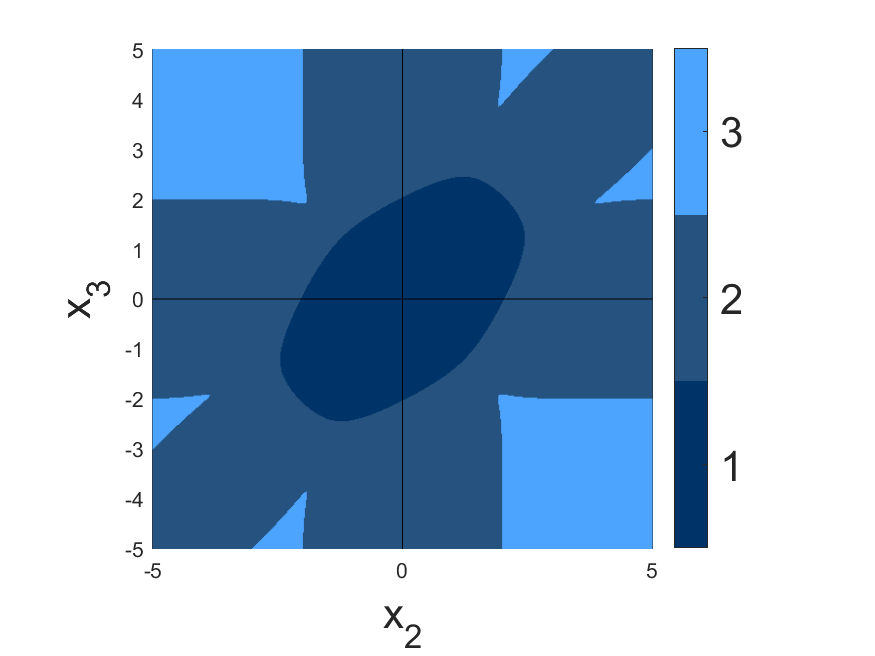
\includegraphics[width=\textwidth]{normal_flag_graph.png}
			\caption{Normal component density with fixed variance $\sigma^2 = 1$.}
			\label{fig:normal_flag_graph}
		\end{subfigure}
		\begin{subfigure}[t]{0.49\textwidth}
			\centering
			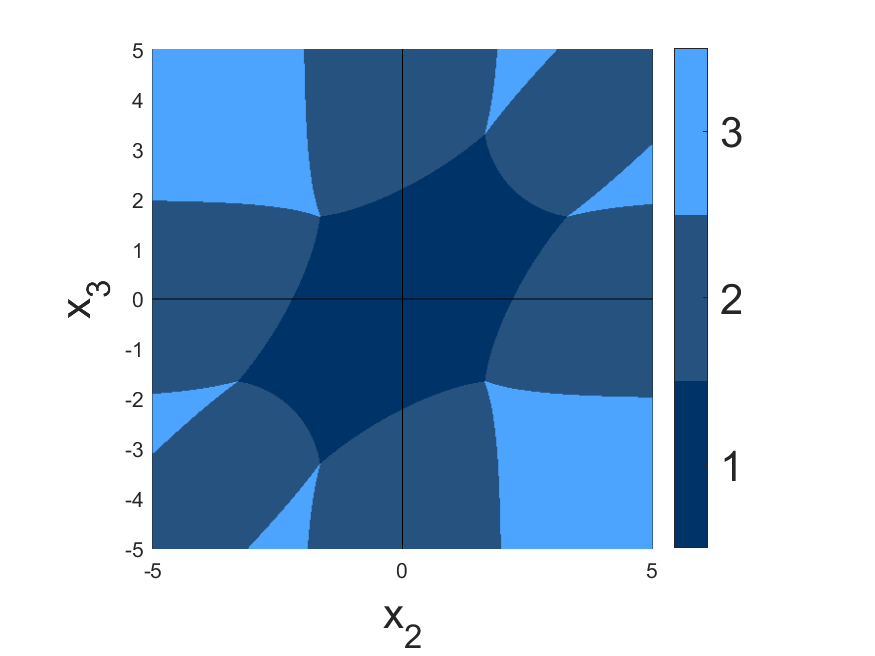
\includegraphics[width=\textwidth]{cauchy_flag_graph.png}
			\caption{Cauchy component density with fixed scale $\gamma = \sqrt{3}$.}
			\label{fig:cauchy_flag_graph}
		\end{subfigure}
		\caption{$K_\vect{x}$ as a function of $\vect{x} = (0, x_2, x_3)$ for two different component densities.}
	\end{figure}
	
	While $n = 2,3$ is not a very realistic scenario when it comes to real data to which we may wish to fit a mixture model, it does help demonstrate a particular way of thinking about the problem of determining $K_\vect{x}$. That is, that $K_\vect{x}$ is simply a function of where $\vect{x}$ lies in $\mathbb{R}^n$. For a particular choice of component density, we can partition $\mathbb{R}^n$ into sets 
	\begin{equation}
		C_k = \{ \vect{x} \in \mathbb{R}^n | K_{\vect{x}} = k \}, \hspace{40pt} k = 1,\dots,n.
		\label{eq: C_k partition sets}
	\end{equation}
	The problem of determining $K_{\vect{x}}$ is then the same as determining in which of the sets $C_k$ $\vect{x}$ lies. If $\vect{x} = \vect{X}$ is randomly chosen, then the probability that $K_\vect{X} = k$ is simply the probability that $\vect{X} \in C_k$. In Section \ref{sec:mixture results}, we present various results which bound the regions $C_k$ in various settings.

	We have attempted to compare the sizes of shapes of the sets $C_k$ for $n = 2$ for the normal and Cauchy densities in Figure \ref{fig:compare cauchy norm flag graph}. In this figure we have plotted $(K_\vect{x}^\mathrm{norm} + K_\vect{x}^\mathrm{Cauchy}) / 2$ to create the effect of overlaying Figures \ref{fig:normal_flag_graph} and \ref{fig:cauchy_flag_graph} (we suggest using these figures as reference to aid readability). We observe in this example that although $C_1^\mathrm{norm} \subset C_1^\mathrm{Cauchy}$, $C_2^\mathrm{norm}$ contains points outside of $C_2^\mathrm{Cauchy}$.


	% \subsection{Other interesting things}
	% We end our empirical results section with 

	% [PUT MORE RESULTS IN HERE]

	\begin{figure}
		\centering
		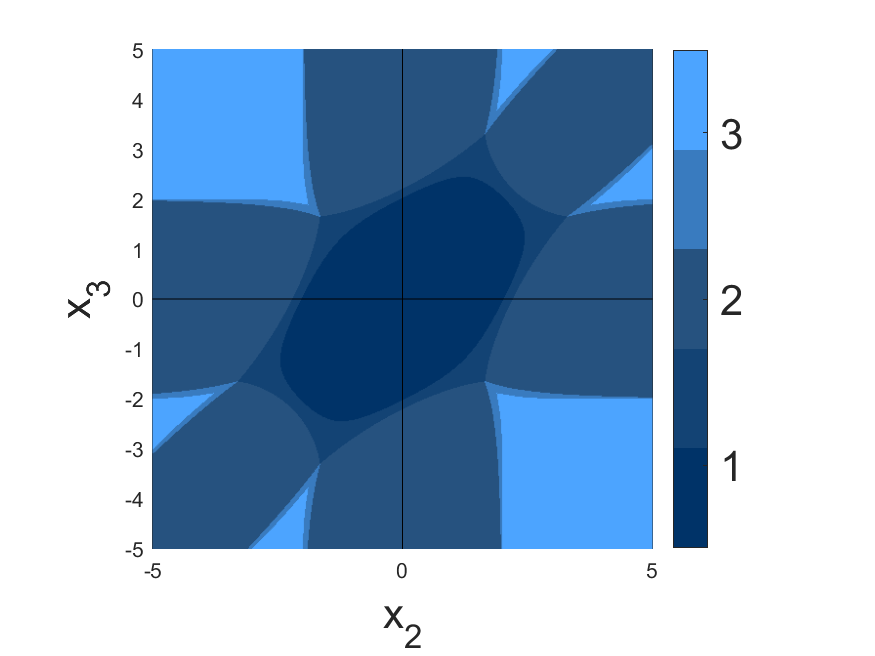
\includegraphics[width = \textwidth]{Figures/Mixtures/norm_cauchy_compare_flag_graph.png}
		\caption{$(K_\vect{x}^\mathrm{norm} + K_\vect{x}^\mathrm{Cauchy}) / 2$}
		\label{fig:compare cauchy norm flag graph}
	\end{figure}

	\section{Results}
		\label{sec:mixture results}
		The figures obtained in Section \ref{sec:empirical results}, as well as the examples in Figures \ref{fig:chi2 n500 motivation} and \ref{fig:collapsing distribution}, suggest that the bounds on $K_\vect{x}$ from Section \ref{sec:summary of Lindsay} could be significantly tightened for location mixtures. The main bounds that we have discussed so far are Theorem \ref{thm: lindsay no more than n points} which states that under mild conditions, $K_\vect{x} \leq n$; and Theorem \ref{thm:exponential family k=1 bound} which provides a sufficient condition for $K_\vect{x} = 1$ for component densities in the exponential class of densities. In this section we will present new bounds on $K_\vect{x}$ that either tighten these bounds, or extend them to different classes of component densities.

		\subsection{Results for \texorpdfstring{$n = 2$}{n = 2}}
		\label{sec:results for n = 2}
		The first bound we present is Theorem \ref{thm:n=2 inflection result} which extends Theorem \ref{thm:exponential family k=1 bound} to a different class of component densities in the case that $n=2$, and which tightens the result to be both sufficient and necessary on this class. The theorem concerns component densities, $f(x)$, which satisfy the assumptions,

		\begin{assumption}[Continuity]
		\label{assump:reallinesupport}
			The density $f(x)$ is continuous and is supported on the whole real line.
		\end{assumption}

		\begin{assumption}[Differentiability]
		\label{assump:twicediff}
			The first and second derivatives of $f(x)$ exist and are continuous.
		\end{assumption}
		
		\begin{assumption}[Unimodality]
			The density $f(x)$ has a single mode at $x=0$. That is, $f'(x) > 0$ for $x <0$, $f'(0) = 0$, and $f'(x) < 0$ for $x>0$.
			\label{assump:singlemode}
		\end{assumption}
		
		\begin{assumption}[Symmetry]
			The density $f(x)$ is symmetric about $x = 0$.
			\label{assump:symmetric}
		\end{assumption}
		
		\begin{assumption}
			The density $f(x)$ has only two points of inflection, located at $x = \pm a$.
			% For some $a > 0$, $f''(-a) = f''(a) = 0$ and these are the only zeros of $f''$.
			\label{assump:twoinflectionpoints}
		\end{assumption}

		% \begin{assumption}		
		% \label{assump:non-zero derivatives}
		% 	The derivative $f'(x)$ is non-zero for all $x \in \mathbb{R}$.
		% \end{assumption}

			
			% \begin{definition}
			% 	If $f$ satisfies assumptions \ref{assump:reallinesupport} through to \ref{assump:singlemode}, then define $[i^-,i^+]$ to be the largest interval that contains 0 and on which $f''(x) \leq 0$.
			% 	\label{def:i-i+}
			% \end{definition}
			% That is, $i^-$ and $i^+$ are inflection points of $f$. Note that for any $f$ satisfying \ref{assump:symmetric}, $i^- = -i^+$. In this case we will write $i = i^+ = -i^-$.
		
		\begin{assumption}
			The density $f(x)$ satisfies $f'(x) < -f'(x - 2a)$ for $x \in (a,\infty)$.
			\label{assump:magnitudegradients}
		\end{assumption}

		\begin{theorem}
			\label{thm:n=2 inflection result}
			Let $f(x)$ satisfy assumptions \ref{assump:reallinesupport} through to \ref{assump:magnitudegradients}. Let $\vect{x} = (x_1,x_2)$ be the sample for which we a finding a maximum likelihood location mixture using $f$ as the component density. Then 
			\begin{equation}
				K_\vect{x} = K(\vect{x};f) = 
					\begin{cases}
						1, &|x_2 - x_1| \leq 2a,\\
						2, &\text{otherwise.}
					\end{cases}
			\end{equation}
		\end{theorem}

		The proof of Theorem \ref{thm:n=2 inflection result} will be given in Section \ref{sec:proof of n=2 inflection result} after some discussion concerning how the likelihood curve behaves when $n = 2$.

		
		It is worth verifying that Assumptions \ref{assump:reallinesupport} through to \ref{assump:magnitudegradients} are satisfied by some common densities. In particular they are satisfied by the common unimodal densities in Table \ref{tab:component densities},
		% We remark here on the following common unimodal densities:
		\begin{align}
			% &\text{Normal with variance $\sigma^2$} && 
			f_\mathrm{norm}(x) &= \frac{1}{\sigma\sqrt{2\pi}} \euler^{-x^2/(2\sigma^2)},\\
			% &\text{Cauchy with scale $\gamma$} && 
			f_\mathrm{Cauchy}(x) &= \frac{1}{\pi (\gamma + x^2/\gamma)}.
			% &\text{Student's t-distribution with $\nu$ degrees of freedom} && f(x) = (1 + x^2/\nu)^{-\frac{\nu + 1}{2}}
		\end{align}
		Clearly, Assumptions \ref{assump:reallinesupport} through to \ref{assump:symmetric} are satisfied for both $f_\mathrm{norm}(x)$ and $f_\mathrm{Cauchy}(x)$.
		The inflection points of $f_\mathrm{norm}(x)$ are located at $x = \pm \sigma$ and the inflection points of $f_\mathrm{Cauchy}(x)$ are located at $x = \pm \gamma/\sqrt{3}$, satisfying Assumption \ref{assump:twoinflectionpoints}. A plot of $f_\mathrm{norm}'(x)$ against $-f_\mathrm{norm}'(x - 2\sigma)$ and of $f_\mathrm{Cauchy}'(x)$ against $-f_\mathrm{Cauchy}'(x - 2\gamma/\sqrt{3})$ in Figure \ref{fig:assumption6} makes it clear that Assumption \ref{assump:magnitudegradients} is satisfied too. Of course, one could make this rigourous if desired.

		\begin{figure}
			\centering
			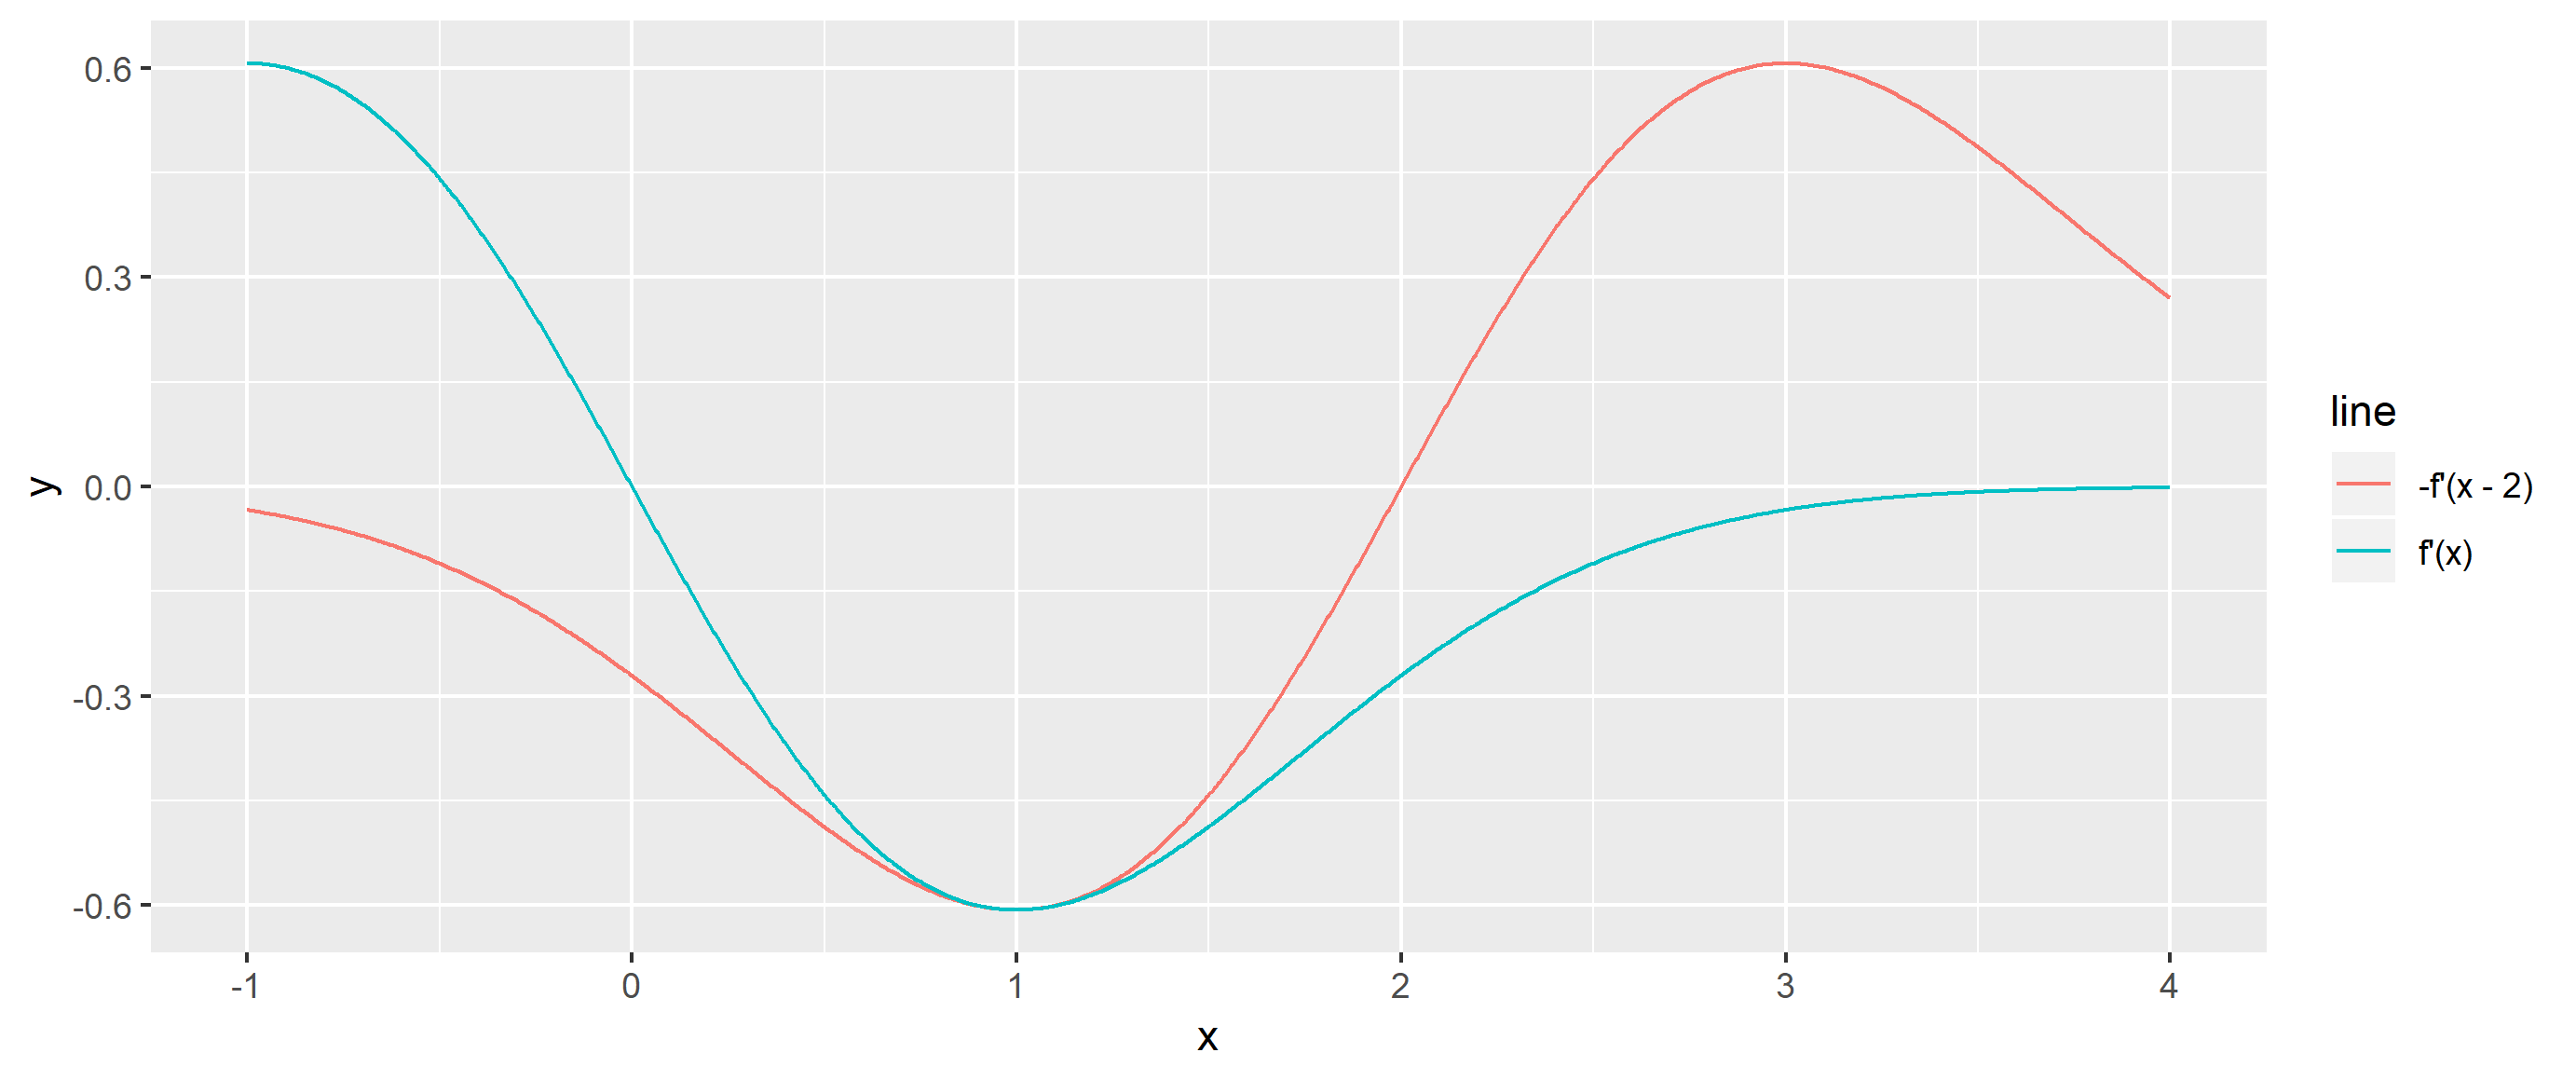
\includegraphics[width = \textwidth]{Figures/Mixtures/assumption6_normal.png}
			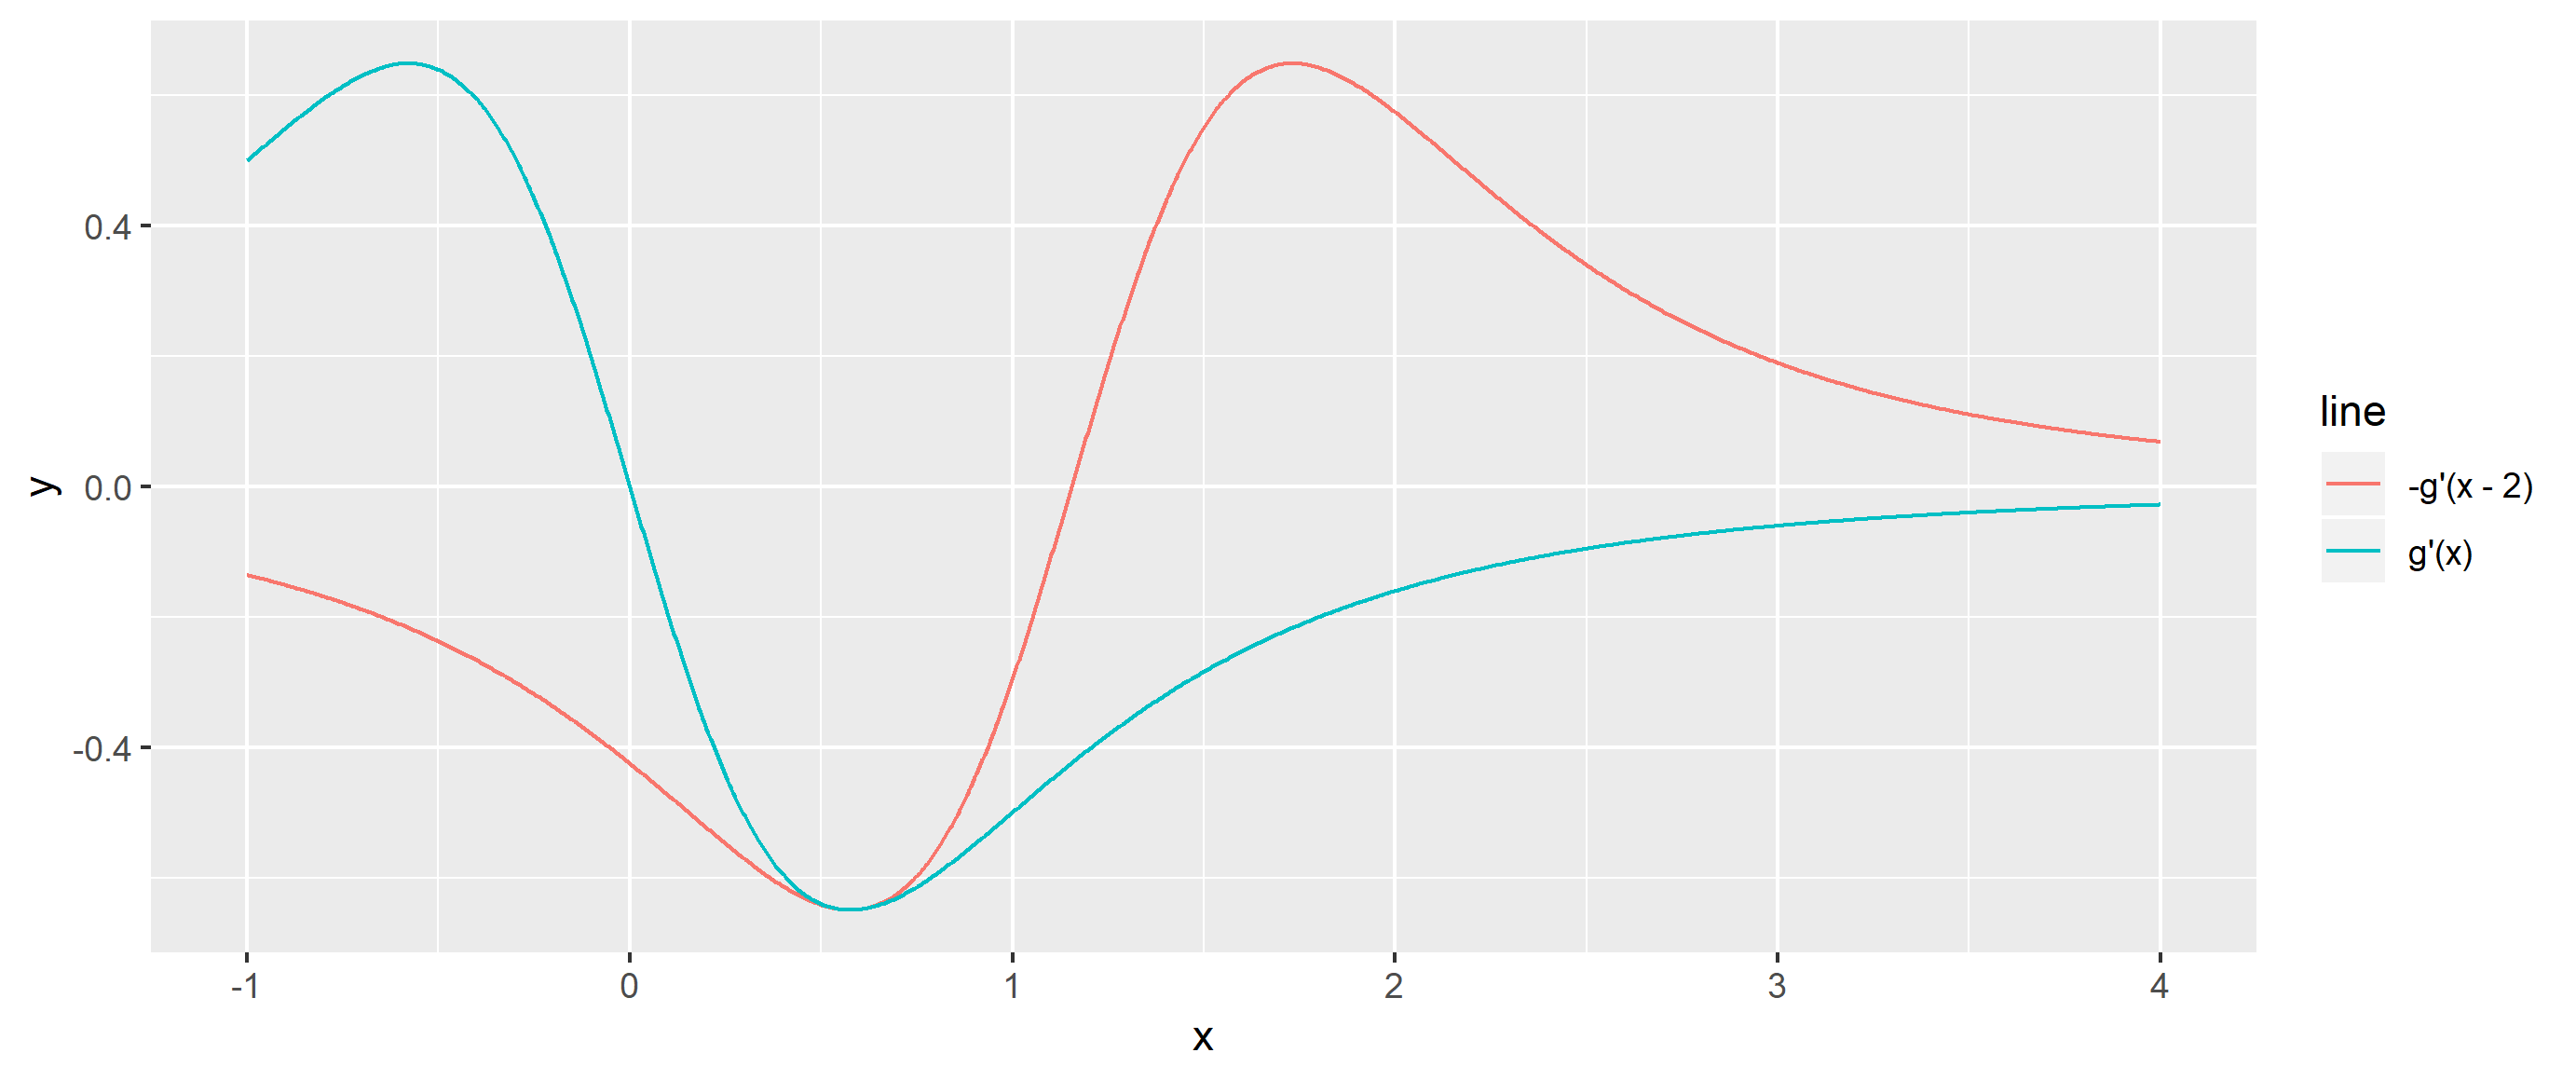
\includegraphics[width = \textwidth]{Figures/Mixtures/assumption6_cauchy.png}
			\caption{Plots of $f_\mathrm{norm}'(x)$ against $-f_\mathrm{norm}'(x - 2\sigma)$ and $f_\mathrm{Cauchy}'(x)$ against $-f_\mathrm{Cauchy}'(x - 2\gamma/\sqrt{3})$ for $\sigma = 1$ and $\gamma = 1$.}
			\label{fig:assumption6}
		\end{figure}
		% We do this in the following Lemma.

		% \begin{lemma}
		% 	The following densities satisfy Assumptions \ref{assump:reallinesupport} through to \ref{assump:magnitudegradients}:
		% 	\begin{align}
		% 		&\text{Normal with variance $\sigma^2$} && f(x) = \frac{1}{\sigma\sqrt{2\pi}} \euler^{-x^2/(2\sigma^2)}\\
		% 		&\text{Cauchy with scale $\gamma$} && g(x) = \frac{1}{\pi (\gamma + x^2/\gamma)}
		% 		% &\text{Student's t-distribution with $\nu$ degrees of freedom} && f(x) = (1 + x^2/\nu)^{-\frac{\nu + 1}{2}}
		% 	\end{align}
		% \end{lemma}
		% \begin{proof}
		% 	Clearly, Assumptions \ref{assump:reallinesupport} through to \ref{assump:symmetric} are satisfied for both $f(x)$ and $g(x)$.

		% 	The inflection points of $f(x)$ are located at $x = \pm \sigma$ and the inflection points of $g(x)$ are located at $x = \pm \gamma/\sqrt{3}$. A plot of $f'(x)$ against $-f'(x - 2\sigma)$ and of $g'(x)$ against $-g'(x - 2\sigma)$ makes it clear that Assumption \ref{assump:magnitudegradients} is satisfied too. 
		% \end{proof}

		% [DISCUSSION RELATING THEOREM TO THE LINDSAY EXPONENTIAL FAMILY ONE]

	
	
		% \begin{assumption}[Continuity]
		% 	$f(x)$ is a continuous density and has the whole real line as its support.
		% 	\label{assump:reallinesupport}
		% \end{assumption}
		
		% \begin{assumption}[Differentiability]
		% 	$f(x)$ is twice differentiable.
		% 	\label{assump:twicediff}
		% \end{assumption}
		
		% \begin{assumption}[Unimodality]
		% 	$f(x)$ has a single mode at $x=0$. I.e. $f'(x) > 0$ for $x <0$, $f'(0) = 0$, and $f'(x) < 0$ for $x>0$.
		% 	\label{assump:singlemode}
		% \end{assumption}
		
		% \begin{assumption}[Symmetry]
		% 	The density $f(x)$ is symmetric about $x = 0$.
		% 	\label{assump:symmetric}
		% \end{assumption}
		
		% \begin{assumption}
		% 	$f$ has only two points of inflection
		% 	\label{assump:twoinflectionpoints}
		% \end{assumption}
		
		% \begin{definition}
		% 	If $f$ satisfies assumptions \ref{assump:reallinesupport} through to \ref{assump:singlemode}, then define $[i^-,i^+]$ to be the largest interval that contains 0 and on which $f''(x) \leq 0$.
		% 	\label{def:i-i+}
		% \end{definition}
		% That is, $i^-$ and $i^+$ are inflection points of $f$. Note that for any $f$ satisfying \ref{assump:symmetric}, $i^- = -i^+$. In this case we will write $i = i^+ = -i^-$.
		
		% \begin{assumption}
		% 	$f'(x) > -f'(x - 2i)$ for $\theta \in (i,\infty)$
		% 	\label{assump:magnitudegradients}
		% \end{assumption}
		
		% Some common densities that satisfy these assumptions include the normal density and the Cauchy density.

		% [WHAT ABOUT IF $N>2$ AND ALL POINTS WITHIN DISTANCE 2I?]

		\subsection{Proof of Theorem \ref{thm:n=2 inflection result}}
		The proof of Theorem \ref{thm:n=2 inflection result} is based on the discussion contained in \cite[Section 4]{Lindsay1983a-he}, in which Lindsay discussed how the curvature of $\Gamma$ relates to the support points of $\hat{Q}$. The important realisation we use here is that points of support must correspond to regions of non-negative curvature of $\Gamma$.

		\label{sec:proof of n=2 inflection result}
		\begin{proof}
			% Since $f(x)$ has a single mode at $x = 0$, the points of support of the maximizing mixing distribution must lie between $x_{1}$ and $x_{2}$. Hence we are
			If $x_1 = x_2$ then clearly $K_\vect{x} = 1$. Otherwise, without loss of generality, assume $x_1 < x_2$. By the unimodality of $f$ (\ref{assump:singlemode}), the points of support of any maximizing mixing distribution, $\hat{Q}$, must lie between $x_1$ and $x_2$ \cite[Proposition 25]{Lindsay1995-sq}. Hence $\hat{\vect{\gamma}} = \vect{\gamma}(\hat{Q}, \vect{x}, f)$ must lie in the convex hull of $\Gamma^*_{\vect{x}, f} = \{\vect{\gamma}(\theta; \vect{x}, f) : \theta \in [x_1, x_2]\}$. 

			Consider the behaviour of $\vect{\gamma}(\theta; \vect{x}, f) = (f(x_1 - \theta), f(x_2 - \theta))$ as we increase $\theta$ from $x_1$ to $x_2$. Since $f(x)$ has a single mode at $x = 0$, $f(x_1 - \theta)$ is non-increasing and $f(x_2 - \theta)$ is non-decreasing along this interval. So $\vect{\gamma}(\theta;\vect{x}, f)$ crosses the line $\gamma_1 = \gamma_2$ once only and by the symmetry of $f(x)$, this occurs at $\theta = (x_1 + x_2)/2$. By Lemma \ref{lemma: maximizing point on line u = v}, we also know that $\hat{\vect{\gamma}}$ must lie on the line $\gamma_1 = \gamma_2$.

			Since $f$ is continuous and twice differentiable, $\vect{\gamma}$ traces out a continuous, smooth curve. The signed curvature
			\begin{align}
				k(\theta) = \frac{-f'(x_1 - \theta)f''(x_2 - \theta) + f'(x_2 - \theta)f''(x_1 - \theta)}{(f'(x_1 - \theta)^2 + f'(x_2 - \theta)^2)^{\frac{3}{2}}}
			\end{align}
			is defined everywhere since $f'(x)$ is zero only at $x = 0$ and so for $x_1 \neq x_2$, the denominator is non-zero everywhere. The sign of $k(\theta)$ matches the sign of
			\begin{equation}
				S(\theta) = 
				\begin{vmatrix}
					\gamma_1'(\theta;\vect{x})&\gamma_1''(\theta;\vect{x})\\
					\gamma_2'(\theta;\vect{x})&\gamma_2''(\theta;\vect{x})
				\end{vmatrix} = 
				\begin{vmatrix}
					-f'(x_1 - \theta) & f''(x_1 - \theta)\\
					-f'(x_2 - \theta) & f''(x_2 - \theta)
				\end{vmatrix}.
			\end{equation}

			Recall from Section \ref{sec: support hyperplane}, that each point of support of a maximizing mixture $\hat{Q}$, corresponds with a contact point of $\Gamma_{\vect{x}, f}$ with the support hyperplane of $\conv(\Gamma_{\vect{x}, f})$ that contains $\hat{\vect{\gamma}}$. Note that any point $\vect{\gamma}(\theta_j;\vect{x},f)$ that is in contact with a support hyperplane of $\conv(\Gamma_{\vect{x}, f})$ must have non-negative curvature.

			First, let us assume that $x_2 - x_1 > 2a$. By the symmetry of $f$, $\vect{\gamma}(\theta;\vect{x})$ crosses the $u_1 = u_2$ line at $\theta = (x_1 + x_2)/2$. At this point, the curvature of $\vect{\gamma}$ has the same sign as
			\begin{equation}
				S\left(\frac{x_1+x_2}{2}\right) = 
				\begin{vmatrix}
					-f'(\frac{x_1 - x_2}{2}) & f''(\frac{x_1 - x_2}{2})\\
					-f'(\frac{x_2 - x_1}{2}) & f''(\frac{x_2 - x_1}{2})
				\end{vmatrix}.
			\end{equation}
			Since $x_2 - x_1 > 2a$, by \ref{assump:twoinflectionpoints},  $f''((x_2 - x_1)/2)>0$. Similarly, $f''((x_1 - x_2)/2) > 0$. We also have that $-f'((x_1 - x_2)/2) < 0$ and $-f'((x_2 - x_1)/2) > 0$. Hence $S((x_1 + x_2)/2)<0$ and so $\vect{\gamma}((x_1 + x_2)/2;\vect{x})$ has negative curvature. Since $\vect{\gamma}$ has negative curvature when it crosses the line $\gamma_1 = \gamma_2$, and since $\hat{\gamma}$ lies on that line, the maximizing point $\hat{\gamma}$ must be the convex combination of at least two separate points in $\Gamma_{\vect{x},f}$ and so $K_\vect{x} = 2$.

			% By Lemma \ref{lemma: gamma has non-negative curvature at points of support} the curve $\Gamma$ cannot have negative curvature at the points of support and so we cannot have that $K_\vect{x} = 1$.
			
			Now assume that $x_2 - x_1 \leq 2a$. By Lemma \ref{lem:magnitudegradients}, there is only one point at which $\vect{\gamma}$ is pointing along the direction $(1,-1)$. Now, by the symmetry of $f$, $\Gamma_{\vect{x}, f}$ must have a line of symmetry along $\gamma_1 = \gamma_2$. Since $\hat{\vect{\gamma}}$ lies on the line $\gamma_1 = \gamma_2$ by Lemma \ref{lemma: maximizing point on line u = v}, the support line of $\Gamma_{\vect{x},f}$ that contains $\hat{\vect{\gamma}}$ must point along the direction $(1, -1)$. Each contact point of $\Gamma_{\vect{x}, f}$ with one of its support lines must be tangent to that support line. Hence, there is only one possible point of contact with the support line that contains $\hat{\vect{\gamma}}$ and so $K_\vect{x} = 1$.

			% [JUST USE SUPORT HYPERPLANE WHICH MUST BE PARALLEL TO u1 = -u2]

			% By the symmetry of $f$ this occurs when $\gamma(\theta;\vect{x})$ is crossing the line $u_1 = u_2$. Since $f$ is continuous, the direction that $\gamma(\theta;\vect{x})$ is moving is also continuous. At $\theta = x_1$, $\gamma(\theta;\vect{x})$ is pointing straight up and so we have that for $\theta \in [x_1,(x_1 + x_2)/2]$, $\gamma(\theta;\vect{x})$ is travelling in a direction pointing above the line perpendicular to $u_1 = u_2$. For $\theta \in [(x_1 + x_2)/2,x_2]$, $\gamma(\theta;\vect{x})$ points below the line. It is now obvious that $\gamma((x_1 + x_2)/2;\vect{x})$ is the furthest point from the origin that lies on $u_1 = u_2$ and is in the convex hull of $\Gamma_\vect{x}$. Since the likelihood increases as we move away from the origin along the line $u_1 = u_2$ in the positive quadrant, we must have
			% $$\hat{\vect{u}} = \gamma((x_1 + x_2)/2;\vect{x})$$
			% and so $K_\vect{x} = 1$.
			
			% Basic idea just here - 		
			% Now either made up of two points or lies on $\Gamma_\vect{x}$. If made up of two points then these two points are symmetrical about $u_1 = u_2$ and the part of $\Gamma_\vect{x}$ that crosses $u_1 = u_2$ is closer to origin. However, if angle of $\gamma$ is always above angle that is perpendicular to $u_1 = u_2$ before crossing $u_1 = u_2$ then impossible for point where it crosses to be closer to origin than that of line between any two symmetrical points.
		\end{proof}

		\begin{lemma}
		\label{lemma: maximizing point on line u = v}
			Let $f(x)$ be a component density symmetric around $x = 0$, and $\vect{x} = (x_1, x_2) \in \mathbb{R}^2$ such that the conditions of Theorem \ref{thm: lindsay maximizing likelihood vector point} are met. Let $\hat{Q}$ maximise the likelihood, $l(Q; \vect{x}, f)$. Then $f_{\hat{Q}}(x_1) = f_{\hat{Q}}(x_2)$.
		\end{lemma}
		\begin{proof}
			Let $(u, v)$ denote the coordinates of $\hat{\vect{\gamma}}  = (f_{\hat{Q}}(x_1), f_{\hat{Q}}(x_2))$. By Theorem \ref{thm: lindsay no more than n points} we have
			\begin{align}
				(u, v) &= p \vect{\gamma}(\theta_1; \vect{x}, f) + (1 - p) \vect{\gamma}(\theta_2;\vect{x}, f)\\
					&= p (f(x_1 - \theta_1), f(x_2 - \theta_1)) + (1 -p) (f(x_1 - \theta_2), f(x_2 - \theta_2))
			\end{align}
			for some choice of $p \in (0, 1]$, and $\theta_1, \theta_2 \in \mathbb{R}$. By the symmetry of $f(x)$, $f(x) = f(-x)$ and so
			\begin{align}
				u &= p f(x_1 - \theta_1) + (1 - p)f(x_1 - \theta_2)\\
					&= p f(\theta_1 - x_1) + (1 - p)f(\theta_2 - x_1)\\
					&= p f(x_2 - [x_1 + x_2 - \theta_1]) + (1 - p) (f(x_2 - [x_1 + x_2 - \theta_2])
			\end{align}
			and likewise
			\begin{align}
				v &= p f(x_1 - [x_1+x_2 - \theta_1]) + (1 - p) f(x_1 - [x_1 + x_2 - \theta_2]).
			\end{align}
			Hence the point $(v, u)$ can be written as
			\begin{align}
				(v, u) = p \vect{\gamma}(x_1 + x_2 - \theta_1;\vect{x}, f) + (1 - p) \vect{\gamma}(x_1 + x_2 - \theta_2;\vect{x}, f),
			\end{align}
			and so $(v, u) \in \conv(\Gamma_{\vect{x}, f})$.
			Since both $(u, v), (v, u) \in \conv(\Gamma_{\vect{x}, f})$, we must have that $\frac{1}{2}(u+v, u + v) \in \conv(\Gamma_{\vect{x}, f})$. Now
			\begin{align}
				\mathcal{L}\left(\frac{1}{2}(u+v, u + v)\right) &= 2\ln((u+v)/2)\\
					&= \ln\left(\left(\frac{u+v}{2}\right)^2\right)\\
					&\geq \ln(uv)\\
					&= \mathcal{L}(u,v).
			\end{align}
			However, $(u, v) = \hat{\vect{\gamma}}$, which by Theorem \ref{thm: lindsay maximizing likelihood vector point} is the unique maximizing point of $\mathcal{L}$ in $\conv(\Gamma_{\vect{x}, f})$. Hence $(u, v) = \frac{1}{2}(u+v, u+v)$ and so $u = v$.
		\end{proof}

		% \begin{lemma}
		% \label{lemma: gamma has non-negative curvature at points of support}
		% 	If $f(x)$ satisfies some stuff then the points of support can only be where the curvature is non-negative.
		% \end{lemma}
		% \begin{proof}
		% 	[DO PROOF]
		% \end{proof}

		\begin{lemma}
			\label{lem:magnitudegradients}
			% Prove stuff about magnitude of gradients (i.e. $\gamma_x < \gamma_y$)
			Let $f(x)$ be a density which satisfies assumptions \ref{assump:reallinesupport} through to \ref{assump:magnitudegradients} and whose inflection points are at $x=a$ and $x=-a$. If 
			$x_2 - x_1 < 2a$ ($x_2 > x_1$) then the equation
			\begin{equation}
				-f'(x_1 - \theta) = f'(x_2 - \theta)
				\label{eq:gradientsequal}
			\end{equation}
			has only one solution.
		\end{lemma}
		\begin{proof}
			We first consider the shape of $f'(x)$. Assumption \ref{assump:singlemode} tells us that $f'(x)$ is positive for $x<0$ and negative for $x>0$. 
			From Assumption \ref{assump:twoinflectionpoints}, the function $f'(x)$ will have turning points at $\pm a$ and these will be the only turning points.
			% From Assumption \ref{assump:twoinflectionpoints}, its derivative, $f''(x)$, satisfies $f''(-a) = f''(a) = 0$ and these are the only zeros of $f''$.
			Hence we have the following picture of $f'(x)$:
			\begin{equation}
				f'(x) \text{ is } 
				\begin{cases}
					\text{positive and increasing,} &x \in (-\infty,-a)\\
					\text{positive and decreasing,} &x \in (-a,0)\\
					\text{negative and decreasing,} &x \in (0,a)\\
					\text{negative and increasing,} &x \in (a,\infty).
				\end{cases}
			\end{equation}
			We also note, from \ref{assump:symmetric}, that $f'(x)$ is an odd function. Using this and rearranging \eqref{eq:gradientsequal} we obtain the equivalent equation
			\begin{equation}
				g(\theta) = h(\theta)
				\label{eq:gradientsequalequivalent}
			\end{equation}
			where we have put $g(\theta) = f'(\theta)$ and $h(\theta) = -f'(\theta - (x_2 - x_1))$ for ease of notation.
			% We now make the assumption that $0<x_2 - x_1<2i$
			% Since $x_2 > x_1$, the right hand side of \eqref{eq:gradientsequalequivalent} is $-f'(x)$ translated to the right by $x_2 - x_1$. Since $x_2 - x_1 < 2i$, the positive turning point of $-f'(\theta - (x_2 - x_1))$ satisfies
			% \begin{equation}
			% -i + x_2 - x_1 < i,
			% \end{equation}
			% that is, it comes before the positive turning point of $f'(\theta)$.
			
			If we assume that $0< x_2 - x_1 < 2a$ then we can consider possible solutions to \eqref{eq:gradientsequalequivalent} on each of the following intervals. 
			
			For $\theta \in (-\infty, 0]$, $g(\theta)\geq 0$ and $h(\theta) < 0$ and so there are no possible solutions.
			
			Likewise, for $\theta \in [x_2 - x_1,\infty)$, $g(\theta)<0$ and $h(\theta) \geq 0$ and so there are no possible solutions.
			
			For $\theta \in [-a + x_2 - x_1, a]$, $g(\theta)$ is decreasing and $h(\theta)$ is increasing and $h(-a +x_2 -x_1) = g(a)$ (since $f'$ is odd). Therefore there must be exactly one solution in this interval.
			
			We note that if $x_2 - x_1 \leq a$ then the above intervals cover the real line. In the case that $a <x_2 - x_1 < 2a$ we need to consider additional intervals.

			For $\theta \in (a,x_2 - x_1)$, from assumption \ref{assump:magnitudegradients}, $f'(\theta) < -f'(\theta - 2a) < -f'(\theta - (x_2 - x_1))$ since both $-f'(\theta - 2a)$ and $-f'(\theta - (x_2 - x_1))$ are increasing on this interval. Hence there can be no solutions to \eqref{eq:gradientsequalequivalent} on this interval.
			
			For $\theta \in (0, -a+x_2 - x_1)$ we can again use assumption \ref{assump:magnitudegradients} by observing that since 
			\begin{equation}
				f'(\theta) < -f'(\theta - 2a)
			\end{equation}
			for $\theta \in (a, \infty)$, we also have that for $\theta \in (-\infty, -a)$
			\begin{equation}
				f'(-\theta) < -f'(-\theta - 2a)
			\end{equation}
			and so for $\theta \in (-\infty, a)$,
			\begin{equation}
				f'(-\theta + 2a) < -f'(-\theta)
			\end{equation}
			which, since $f'$ is odd, is equivalent to 
			\begin{equation}
				-f'(\theta - 2a) < f'(\theta).
			\end{equation}

			So for $\theta \in (0,-a+x_2-x_1)$,  $f'(\theta)>-f'(\theta - 2a) > -f'(\theta - x_2 - x_1)$ and there are no solutions to \eqref{eq:gradientsequalequivalent} on this interval either.
			
			Since the above intervals cover the real line and since we have shown that there is only one solution in one of these intervals, \eqref{eq:gradientsequal} must have only one solution.
		\end{proof}

	\subsection{Results for general \texorpdfstring{$n$}{n}}
	\label{sec: results for general n}
	To obtain results for $n \geq 2$ we now restrict our component density to be normal with fixed variance $\sigma^2$. In this case, we can make use of the gradient function defined in Section \ref{sec: gradient characterization} and equations, \eqref{eq:Deq1} to \eqref{eq:Deq3}, which must be satisfied at a maximizing mixture.

	When our component density is normal with variance $\sigma^2$, that is
	\begin{equation}
		f_\sigma(x) = \frac{1}{\sigma \sqrt{2\pi}} \euler^{-x^2/2\sigma^2},
	\end{equation}
	the gradient function defined in \eqref{eq:def gradient function}, evaluated at a mixture $Q$ which places masses $\vect{p}$ at locations $\vect{\theta}$, becomes
	\begin{equation}
		D_Q(\theta; \vect{x}, f_\sigma) = - n + \sum_{i = 1}^n \frac{\exp({-(x_i - \theta)^2/2\sigma^2})}{\sum_{j=1}^m p_j \exp({-(x_i - \theta_j)^2/2\sigma^2})}.
	\end{equation}
	% where we have written
	% \begin{equation}{}
	% 	\Gamma_k(x;\vect{\theta},\vect{p}) = \frac{f(x - \theta_k;\sigma)}{\sum_{j=1}^m p_j f(x - \theta_j;\sigma)}.
	% \end{equation}
	% for ease of notation. Using this notation, equations \eqref{eq:Deq1} to \eqref{eq:Deq3} become
	Equations \eqref{eq:Deq1} to \eqref{eq:Deq3} state that at a maximizing mixture $\hat{Q}$, 
	\begin{align}
		&\frac{1}{n} \sum_{i=1}^n \Psi_k(x_i;\hat{\vect{\theta}},\hat{\vect{p}}) = 1, &&k = 1,\dots, m, \label{eq:PsiEq1}\\
		&\frac{1}{n} \sum_{i=1}^n x_i \Psi_k(x_i;\hat{\vect{\theta}},\hat{\vect{p}}) = \theta_k, &&k = 1,\dots, m,\label{eq:PsiEq2}\\
		&\frac{1}{n} \sum_{i=1}^n (x_i - \theta_k)^2 \Psi_k(x_i;\hat{\vect{\theta}},\hat{\vect{p}}) \leq \sigma^2, &&k = 1,\dots, m,
		\label{eq:PsiEq3}
	\end{align}
	where $\hat{\vect{\theta}}$ and $\hat{\vect{p}}$ are the locations and masses of $\hat{Q}$ and we have written
	\begin{equation}{}
		\Psi_k(x;\vect{\theta},\vect{p}) = \Psi_k(x;\vect{\theta},\vect{p}, f_\sigma) = \frac{f_\sigma(x - \theta_k)}{\sum_{j=1}^m p_j f_\sigma(x - \theta_j)}
	\end{equation}
	for ease of notation. 

	We will show that these three equations constrain the regions $C_1, \dots, C_n$ as defined in \eqref{eq: C_k partition sets}. This will be done in Theorem \ref{thm:general n constraints result}. However, as a gentle introduction, we will start with the much simpler problem of just bounding $C_1$.

	\begin{theorem}
		\label{thm:general n C1 bound}
		If $\vect{x} \in C_1$ then 
		\begin{equation}
			\frac{1}{n} \sum_{i=1}^n (x_i - \bar{\vect{x}})^2 \leq \sigma^2,
		\end{equation}
		where 
		\begin{equation}
			\bar{\vect{x}} = \frac{1}{n}\sum_{i = 1}^n x_i.
		\end{equation}
	\end{theorem}
	\begin{proof}
		If $\vect{x} \in C_1$ then the maximizing mixture has one component and so $\Psi_1(x; \vect{\theta}, \vect{p}) = 1$. Then \eqref{eq:PsiEq2} gives us that $\theta_1 = \bar{\vect{x}}$ and combining this with \eqref{eq:PsiEq3} completes the proof.
	\end{proof}
	In Figure \ref{fig:flag graph m1 bound} we compare the bound above to the `flag graphs' we produced in section \ref{sec: flag graphs}.

	\begin{figure}
		\centering
		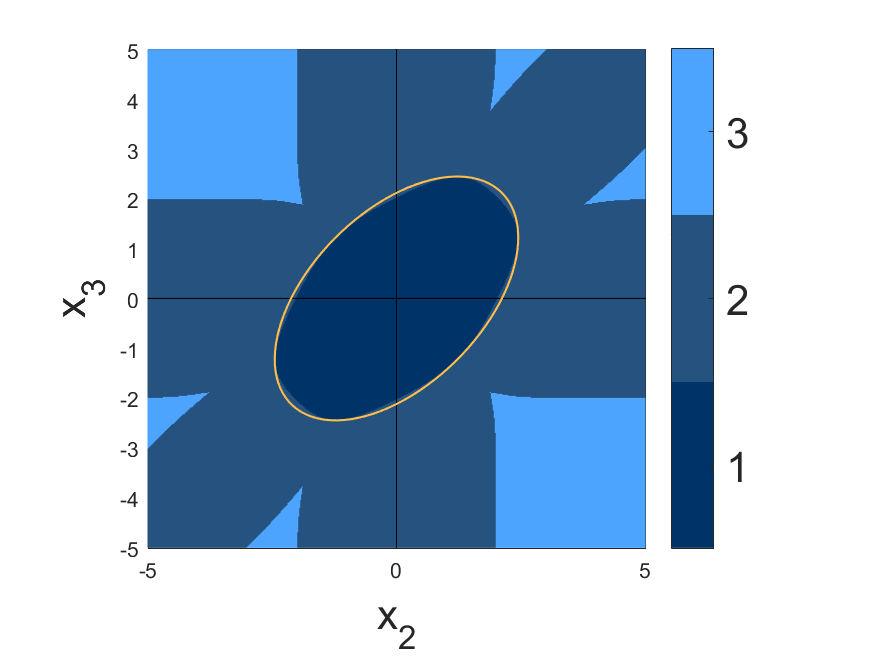
\includegraphics[width = \textwidth]{Figures/Mixtures/normal_flag_graph_m1_bound.png}
		\caption{The bound obtained in Theorem \ref{thm:general n C1 bound} tells us that $C_1$ must lie within the orange ellipse. The true shape of $C_1$ is given by the dark blue region.}
		\label{fig:flag graph m1 bound}
	\end{figure}

		% From Theorem \ref{thm:shapeofC1normalb}, an lower bound to $\prob(\vect{x} \in C_1)$ is
		% \begin{align*}
		% p_l &= \prob(x_{(n)} - x_{(1)} < 2\sigma)\\
		% 	&\geq \prob(\mu - \sigma < x_{(1)} < x_{(n)} < \mu + \sigma )\\
		% 	&=  \left(\int_{\mu - \sigma}^{\mu + \sigma} f(x) \intd x \right)^n\\
		% 	&= \left( \erf\left(\frac{\sigma_2}{\sqrt{2}\sigma_1}\right)\right)^n
		% \end{align*}

	
	% \subsection{Bounding \texorpdfstring{$C_m$}{Cm}}
	We now state a generalisation of Theorem \ref{thm:general n C1 bound} that bounds the regions $C_1, \dots, C_n$.

	\label{sec:bounding Cm}
		\begin{theorem}
			If $\vect{x} \in C_m$ for some $m \leq n$, then there exists a subset of the $x_i$, $A$, such that $A$ contains at least $n/m$ elements and
			\begin{equation}
				\frac{1}{n} \sum_{i \in A} \left(x_i - \bar{x}_A\right)^2 \leq \sigma^2,
			\end{equation}
			where
			\begin{equation}
				\bar{x}_A = \frac{1}{|A|}\sum_{i \in A} x_i.
			\end{equation}
			\label{thm:general n constraints result}
		\end{theorem}
		\begin{proof}
			Let $\hat{\vect{\theta}}$ and $\hat{\vect{p}}$ represent an $m$ point maximizing mixture of $\vect{x} \in C_m$. By Lemma \ref{lem:maxkGamma} below, for every $i \in \{1, \dots, n\}$ there exists a $k \in \{1, \dots, m\}$ such that $\Psi_{k}(x_i;\hat{\vect{p}},\hat{\vect{\theta}}) \geq 1$. Therefore by the pigeonhole principle there must exists some $k^*$ such that $\Psi_{k^*}(x_i;\hat{\vect{p}},\hat{\vect{\theta}}) \geq 1$ for at least $n / m$ different $i$. Define the set
			\begin{equation}
			 	A_{k^*} = \{i : \Psi_{k^*}(x_i;\hat{\vect{p}},\hat{\vect{\theta}}) \geq 1 \},
			\end{equation}
			which we know must have size $|A_{k^*}| \geq n/m$.
			% Let $\vect{x} = (x_1,\dots,x_n)$ and assume that the maximum likelihood mixture for $\vect{x}$ has no more than $m$ components. Let $\hat{\vect{\theta}}$ and $\hat{\vect{p}}$ denote this maximizing mixture. %Let $\hat{\vect{\theta}} = (\hat{\theta}_1,\dots,\hat{\theta}_m)$ and $\hat{\vect{p}} = (\hat{p}_1,\dots,\hat{p}_m)$ be a maximizing mixture for $\vect{x}$
			% Then by Lemma \ref{lem:maxkGamma}, there exists a $k^*$ such that $\Psi_{k^*}(x_i;\hat{\vect{p}},\hat{\vect{\theta}}) \geq 1$ for at least $\lceil \frac{n}{m} \rceil$ different $x_i$. Let $A_{k^*}$ be the set of all these $x_i$. 

			% Let $A_{\theta_{k^*}}$ be the set of the $|A_{k^*}|$ closest $x_i$ to $\theta_{k^*}$. 

			From \eqref{eq:PsiEq3},
			\begin{align}
				\sigma^2 &\geq \frac{1}{n} \sum_{i=1}^n (x_i - \theta_{k^*})^2 \Psi_{k^*}(x_i; \hat{\vect{\theta}}, \hat{\vect{p}})\\ 
					&\geq \frac{1}{n} \sum_{i \in A_{k^*}} (x_i - \theta_{k^*})^2 \Psi_{k^*}(x_i; \hat{\vect{\theta}}, \hat{\vect{p}})\\
					&\geq \frac{1}{n} \sum_{i \in A_{k^*}} (x_i - \theta_{k^*})^2,
					\label{eq:sum A_k^star x_i - theta}
					% &\geq \frac{1}{n} \sum_{i \in A_{\theta_{k^*}}} (x_i - \theta_{k^*})^2 \\
					% &\geq \frac{1}{n} \sum_{i \in A_{k^*}} \left(x_i - \bar{x}_{A_{k^*}}\right)^2.
			\end{align}
			since $\Psi_{k^*}(x_i;\hat{\vect{p}},\hat{\vect{\theta}}) \geq 1$ for all $i \in A_{k^*}$. Finally, we can reduce \eqref{eq:sum A_k^star x_i - theta} by replacing $\theta_{k^*}$ with $\bar{x}_{A_{k^*}}$ to get that
			\begin{equation}
				\sigma^2 \geq \frac{1}{n} \sum_{i \in A_{k^*}} \left(x_i - \bar{x}_{A_{k^*}}\right)^2.
			\end{equation}
			% From \eqref{eq:PsiEq3},
			% \begin{equation}
			% 	\frac{1}{n} \sum_{i \in A_{\theta_{k^*}}} \left(x_i - \bar{x}_{A_{\theta_{k^*}}}\right)^2 \leq \sigma^2.
			% \end{equation}
		\end{proof}

		% This means that if we cannot find a subset of the $x_i$ that has at least $\frac{n}{m}$ elements and has (biased) variance less than $\frac{n\sigma^2}{\left\lceil \frac{n}{m} \right\rceil}$ then we need more than $m$ components in our maximum likelihood mixture.
	% \subsection{Properties of \texorpdfstring{$\Psi$}{Psi}}
	% 	% In order to obtains bounds on the regions $C_2, \dots, C_n$, we will need to get a handle on the behaviour of $\Psi_k(x;\vect{\theta}, \vect{p})$. 
	% 	This section contains statements and proofs of Lemmas concerning the properties of $\Psi$ that are used in the proof of Theorem \ref{thm:general n constraints result}.

		The bound for the $C_2$ region given by Theorem \ref{thm:general n constraints result} is compared to the `flag graphs' from Section \ref{sec: flag graphs} in Figure \ref{fig:flag graph m2 bound}. We observe that the bound does not appear as tight as the one bounding $C_1$.

		\begin{figure}
			\centering
			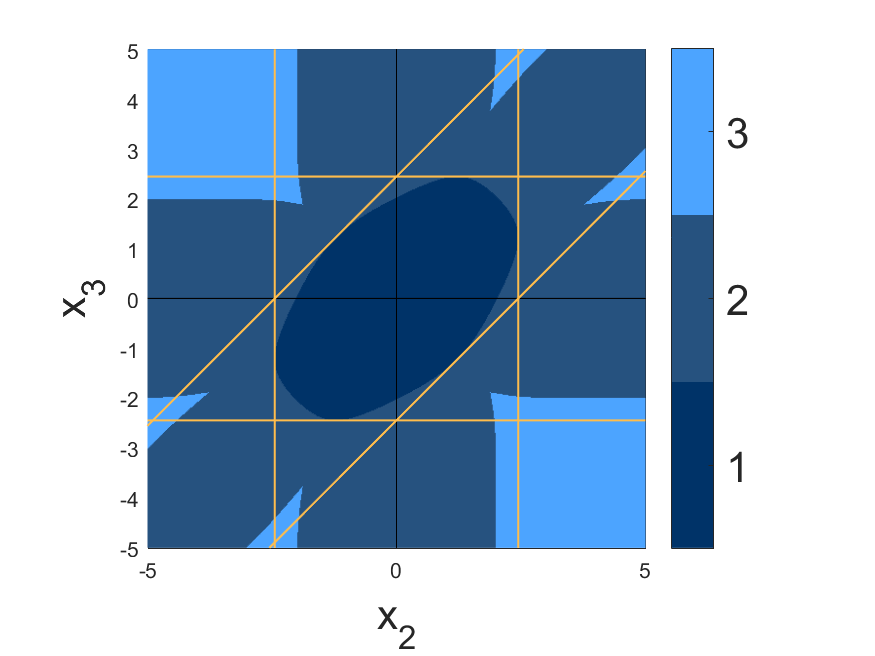
\includegraphics{Figures/Mixtures/normal_flag_graph_m2_bound.png}
			\caption{The bound obtanied in Theorem \ref{thm:general n constraints result} tells us that $C_2$ must lie between the pairs of parallel orange lines. The true shape of $C_2$ is given by the middle blue shaded region.}
			\label{fig:flag graph m2 bound}
		\end{figure}

		\begin{lemma}
		\label{lem:maxkGamma}
		Let $f$ be a density supported on all of $\mathbb{R}$. For all $x \in \mathbb{R}$, and all discrete probability distributions with masses $\vect{p}$ at locations $\vect{\theta}$,
			\begin{equation}
				\max_k \left[ \Psi_k(x;\vect{p},\vect{\theta},f) \right] \geq 1.
			\end{equation}
		\end{lemma}	
		\begin{proof}
			Let $x \in \mathbb{R}$, and $\vect{\theta},\vect{p}$ be the locations and weights respectively of an $m$ point discrete probability distribution. Choose $\theta_{k^*}$ to be the smallest $\theta_j$ that satisfies
			\begin{align}
				f(x - \theta_{k^*}) &\geq f(x - \theta_j) && j = 1, \dots, m.
			\end{align}
			(We choose the smallest in case there is more than one $\theta_j$ which satisfies the above). Then
			\begin{equation}
				\Psi_{k^*}(x;\vect{p},\vect{\theta},f) = \frac{f(x - \theta_{k^*})}{\sum_{j=1}^m p_j f(x - \theta_j)} \geq \frac{f(x - \theta_{k^*})}{\sum_{j=1}^m p_j f(x - \theta_{k^*})} = 1.
			\end{equation}
		\end{proof}

		% \begin{lemma}
		% 	\begin{equation}
		% 	\Psi_k(x;\vect{p},\vect{\theta}) \leq \frac{1}{p_k}
		% 	\end{equation}
		% \end{lemma}
		% \begin{proof}
		% 	Since $f(x) > 0$,
		% 	\begin{equation}
		% 		\Psi_k(x;\vect{p},\vect{\theta}) = \frac{f(x - \theta_k;\sigma)}{\sum_{j=1}^m p_j f(x - \theta_j;\sigma)} \leq \frac{f(x - \theta_k;\sigma)}{p_k f(x - \theta_k;\sigma)} = \frac{1}{p_k}.
		% 	\end{equation}
		% \end{proof}

		% \begin{lemma}
		% 	Let $\gamma(x)$ be a non-negative function that satisfies
		% 	\begin{equation}
		% 		\frac{1}{n} \sum_{i=1}^n \gamma(x_i) = 1.
		% 	\end{equation}

		% 	Then the $\theta$ that minimizes 
		% 	\begin{equation}
		% 		\frac{1}{n} \sum_{i=1}^n (x_i - \theta)^2 \gamma(x_i)
		% 	\end{equation}
		% 	is
		% 	\begin{equation}
		% 		\theta = \frac{1}{n} \sum_{i=1}^n x_i \gamma(x_i).
		% 	\end{equation}
		% \end{lemma}
		% \begin{proof}
		% 	CURRENTLY UNUSED. PROOF IN TIM'S NOTEBOOK.
		% \end{proof}

	\subsection{Treating \texorpdfstring{$\vect{x}$}{x} as random}

		Up until now, we have treated $\vect{x}$ as fixed, not random, and treated the maximum likelihood problem purely as an optimization one, rather than a statistical one. However, for this section we consider a random sample
		\begin{equation}
			\vect{X} = (X_1, \dots, X_n)
		\end{equation}
		where the $X_i$ are i.i.d. with normal distribution 
		\begin{equation}
			X_i \sim N(\mu, \sigma_1^2).
		\end{equation}
		Given a component density, we may consider the probabilities
		\begin{align}
			&\prob[\vect{X} \in C_m],	&&m = 1,\dots,n.
		\end{align}
		
		\begin{theorem}
		\label{thm:probability in C1}
			Let the component density with which we are finding a maximum likelihood location mixture be normal with variance $\sigma_2^2$. Then 
			\begin{equation}
				\prob[\vect{X} \in C_1] \leq \prob\left(\chi_{n-1}^2 \leq \frac{n \sigma_2^2}{\sigma_1^2}\right)
			\end{equation}
			where $\chi_{n-1}^2$ is chi-squared with $n-1$ degrees of freedom.
		\end{theorem}
		\begin{proof}
			From Theorem \ref{thm:general n C1 bound},
			\begin{align}
			\prob\left(\vect{X} \in C_1 \right) &\leq \prob \left( \sum_{i=1}^n (X_i - \bar{\vect{X}})^2 \leq n \sigma_2^2  \right) \\
				&= \prob\left( \frac{1}{\sigma_1^2}\sum_{i=1}^n (X_i - \bar{\vect{X}})^2 \leq \frac{n \sigma_2^2}{\sigma_1^2}\right)\\
				% &= \prob\left( \frac{s^2}{\sigma_1^2} \leq \frac{n \sigma_2^2}{\sigma_1^2}\right)\\
				&= \prob\left(\chi_{n-1}^2  \leq \frac{n \sigma_2^2}{\sigma_1^2} \right).
			\end{align}
		\end{proof}

		Theorem \ref{thm:probability in C1} is of particular interest when the $\sigma_1 = \sigma_2$. In this case, our mixture can select the `true' number of components, which will happen if $\vect{X} \in C_1$. The probability of this occurring satisfies
		\begin{align}
			\prob\left(\vect{X} \in C_1\right) &\leq \prob\left(\chi_{n-1}^2 \leq n\right)
		\end{align}
		which converges to $1/2$ as $n \rightarrow \infty$. This is a simple proof that the number of components chosen by a normal location mixture is not a consistent estimator for the true number of components.

		Similar results to this have already been discovered. In \cite{Hartigan1985-wn}, Hartigan considered the mixture 
		\begin{equation}
			(1 - p)N(0,1) + pN(\theta, 1)
		\end{equation}
		and showed that the likelihood ratio between $\theta = 0$ and $\theta \neq 0$ converges to $\infty$ as $n \rightarrow \infty$. Also related is the result \cite{Leroux1992-ek} that certain penalised likelihoods do not underestimate the true number of components (and so it is reasonable to expect that the unpenalised likelihood might overestimate the true number of components).

		% [SOMETHING RELATED TO RESULT FOR N = 2?]
		%I.E. we can calculate the exact probability for $x \in C_1$ when n = 2... could compare this

		In this section, we have taken advantage of the simple form that the gradient function and its derivatives take when the component density is normal. One might consider using equations \eqref{eq:Deq1} through \eqref{eq:Deq3} to find analogous results for the Cauchy density (which we considered in Section \ref{sec:results for n = 2}) or other densities outside of the normal family. However, we found that the derivatives of the gradient function were too complex to be able generalise these results to other component densities.

	% \subsection{Derive Constraints again}
	% WE SHOULD BE ABLE TO DERIVE \eqref{eq:PsiEq1} THROUGH \eqref{eq:PsiEq3} AGAIN USING THEOREM \ref{thm:solution in interior}.

% \section{Other Results}


	% \subsection{Discussion about what we hope to acheive}
	% 	The few original results above (Theorems \ref{thm:n=2 inflection result} and \ref{thm:general n constraints result}) seem to be special cases of what looks to be a much more general rule. Theorem \ref{thm:general n constraints result} seems to be too large by a factor of $m$ when you compare to numerics, and the distance between inflection points in Theorem \ref{thm:n=2 inflection result} seems to come up again when when you look at images like Figure \ref{fig:normal_flag_graph} (eg the thickness of the `bands' is this distance). It is therefore our hope that we can either generalize or add significantly to the Theorems stated so far.

	% \subsection{Final Observation}
	% [EXTRA STUFF]

	% ``The result follows from this general theorem which seems obvious.''

	% \begin{theorem}
	% 	\label{thm:solution in interior}
	% 	Let $(E_m)_{m=1}^\infty$ be a sequence of subsets of topological spaces and let $(g_m)_{m=1}^\infty, g_m: E_m \mapsto \mathbb{R}$ be a sequence of	functions that satisfy the following properties
	% 	\begin{enumerate}
	% 		\item $\forall \vect{x} \in \partial E_m, \exists n < m, \vect{y} \in E_n$ such that $g_m(\vect{x}) \leq g_n(\vect{y})$.
	% 		\label{prop:one}
	% 		\item $\exists m_0, \vect{x}_0 \in E_{m_0}$ such that $\forall m, \vect{x} \in E_m$, $g_m(\vect{x}) \leq g_{m_0}(\vect{x}_0)$.
	% 	\end{enumerate}
	% 	Then $\exists m_*, \vect{x}_* \in E_{m_*} \setminus \partial E_{m_*}$ such that $\forall m, \vect{x} \in E_m$, $g_m(\vect{x}) \leq g_{m_*}(\vect{x}_*)$.
	% \end{theorem}
	% \begin{proof}
	% 	The proof is simple. If $\vect{x}_0 \notin \partial E_{m_0}$ then we are done. Otherwise, by property \ref{prop:one} we can find a $n$ and $\vect{y} \in E_n$ such that $g_n(y) = g_{m_0}(\vect{x}_0)$. If $\vect{y} \notin \partial E_n$ then we are done, otherwise we repeat the process until we find a $m, \vect{x}$ pair with $\vect{x} \notin \partial E_m$. %Note that property \ref{prop:one} implies that $\partial E_1 = \emptyset$ and so this process must end.
	% \end{proof}

	% The application to the maximum likelihood mixture problem is simple. 

\section{Conclusion}

In this chapter we have analysed the behaviour of the mixing distribution of certain maximum likelihood location mixtures. We were concerned mainly with $K_\vect{x}$ - the number of components in these mixtures, or equivalently, the number of points of support in the corresponding mixing distribution. While bounds on $K_\vect{x}$ existed in the literature, mainly thanks to Lindsay's seminal papers on the geometry of mixture likelihoods, empirical results suggested that in many cases these bounds could be significantly tightened. In exploring these empirical results, we demonstrated that given a component density, we could partition $\mathbb{R}^n$ into sets, $C_m$, based on the number of components that each point $\vect{x} \in \mathbb{R}^n$ required. For small $n$ these could be easily visualized and these plots provided a reference against which to compare any bounds on $K_\vect{x}$.

We proved a number of results providing bounds on $K_\vect{x}$ that to the best of our knowledge are new. For $n = 2$, we found an explicit formula for $K_\vect{x}$ for a certain class of symmetric, unimodal component densities. For $n \geq 2$, we restricted our attention to normal component densities and, for each $m \leq n$, provided a necessary condition for $\vect{x} \in C_m$. We used these bounds to show that the number of components chosen by a normal location mixture is not a consistent estimator for the true number of components. 

Overall, this chapter provided new insights into maximum likelihood location mixtures by treating the problem as an optimization problem, rather than a statistical problem.
% [EXTEND?]
In the next chapter we will examine another optimization problem in statistics which exhibits a similar phenomenon. In it we find a probability mass function as the solution to an optimization problem, and discover that in a large number of cases it is supported on only a few points.